\documentclass[edeposit,mixcasechap,tocnosub,noragright,centerchapter,fullpagesingle,12pt]{uiuc_csthesis21}

% Updated version of the ECE department's latex resources

% Use draftthesis for notes and date markings on every page.  Useful when you
%   have multiple copies floating around.
% Use offcenter for the extra .5 inch on the left side. Needed with fullpage and fancy.
% Use mixcasechap for compatibility with hyperref package, which does NOT like all caps default
% Use edeposit for the adviser/committee on the title page.
% Use tocnosub to suppress subsection and lower entries in the TOC.
% PhD candidates use "proquest" for the proquest abstract.

\makeatletter

\usepackage{setspace}  % Useful for single, 1.5, and double spacing
\usepackage{url}  % Useful for URLs
%\usepackage{hyperref}  % Another package useful for URLs

\usepackage{lscape}  % Useful for wide tables or figures.
% Following command definition is from Stack Exchange: https://tex.stackexchange.com/questions/278113/single-landscape-page-with-page-number-at-the-bottom 
% It adds *rotated* page numbers to the bottom of landscaped pages to meet the Graduate College standards (see page 7 here: https://grad.illinois.edu/files/pdfs/thesis-sample-chapter-straight-numbering.pdf)
\def\fillandplacepagenumber{
	\par
	\pagestyle{empty}
	\vbox to 0pt{\vss}
	\vfill
	\vbox to 0pt{
		\baselineskip 0pt
		\hbox to \linewidth{\hss}
		\baselineskip\footskip
		\hbox to \linewidth{\hfil\thepage\hfil}\vss
	}
}

% {{{ packages

\usepackage{blindtext}

% math
\usepackage{amsmath}
\usepackage{amsthm}
\usepackage{stmaryrd}
\usepackage{cases}
\usepackage{algorithm,algpseudocode}

% pretty links
\usepackage{xparse}
\usepackage{hyperref}
\usepackage[nameinlink]{cleveref}
\hypersetup{
    colorlinks=true,
    urlcolor=blue,
    citecolor=black,
    linkcolor=black
}

\usepackage{listings}
\usepackage{caption}
\usepackage{subcaption}

\usepackage{graphicx}

\usepackage[
    style=apa,
    backend=biber,
    style=numeric ]{biblatex}

% better environments
\usepackage[shortlabels]{enumitem}
\usepackage{booktabs}
\usepackage{caption}
\usepackage{multirow}

% graphics
\usepackage{tikz}
\usetikzlibrary{calc}
\usetikzlibrary{arrows,automata,fit,positioning,shapes}

% fancier font
\usepackage[sc]{mathpazo}
% better typography
\usepackage[activate={true,nocompatibility}, % activate protrusion and font expansion
            final,              % enable microtype, use draft to disable
            tracking=true,
            kerning=true,       % optimise interactions between characters
            spacing=true,       % more uniform spacing between words
            factor=1100,        % more protrusion
            stretch=10,         % smaller values (default 20, 20) to avoid blurring
            shrink=10]{microtype}
\SetTracking{encoding={*}, shape=sc}{40}

% }}}

% {{{ formatting

% enable section numbering only for the first three header levels
\setcounter{secnumdepth}{2}

% caption format
% NOTE: set format=plain to remove caption indentation
\captionsetup{
    format=hang
}

% allow subsubsections in the TOC, if there are any
% NOTE: if you got to subsubsections, you probably have too many!
\setcounter{tocdepth}{\subsubsectiontocdepth}
\setcounter{secnumdepth}{\subsubsectionnumdepth}

% NOTE: if there are many levels of indentation int the TOC, making it flat
% might be a good option with the following options
% \KOMAoption{toc}{indenttextentries,flat}

% https://marketing.illinois.edu/visual-identity/color
\definecolor{IlliniOrange}{RGB}{255, 95, 5}
\definecolor{IlliniAltgeld}{RGB}{200, 65, 19}
\definecolor{IlliniBlue}{RGB}{19, 41, 75}

\definecolor{IlliniAlmaMater}{RGB}{30, 56, 119}
\definecolor{IlliniIndustrialBlue}{RGB}{29, 88, 167}
\definecolor{IlliniArchesBlue}{RGB}{0, 159, 212}
\definecolor{IlliniCloud}{RGB}{248, 250, 252}
\definecolor{IlliniHeritageOrange}{RGB}{245, 130, 30}

% }}}

% {{{ commands

\NewDocumentCommand \dx { O{x} } {\,\mathrm{d} #1}
\NewDocumentCommand \vect { m } { \mathbold{#1} }
\NewDocumentCommand \od { m m } { \dfrac{\mathrm{d} #1}{\mathrm{d} #2} }
\NewDocumentCommand \pd { m m } { \dfrac{\partial #1}{\partial #2} }

% jump notation
\NewDocumentCommand \jump { sm } {
    \IfBooleanTF#1
    {\left\llbracket #2 \right\rrbracket}
    {\llbracket #2 \rrbracket}
}
% average notation
\NewDocumentCommand \avg { sm } {
    \IfBooleanTF#1
    {\left\langle #2 \right\rangle}
    {\langle #2 \rangle}
}
% inner product
\NewDocumentCommand \ip { m } { \avg{ #1 } }

\DeclareMathOperator{\tr}{tr}
\DeclareMathOperator{\sech}{sech}
\DeclareMathOperator{\argmin}{\operatorname{arg}\,\operatorname{min}}

% }}}

% {{{ environments

\NewDocumentCommand \newtheoremin { m m m } {
    \newtheorem{#1}{#2}
    \numberwithin{#1}{#3}
}
\newtheoremin{example}{Example}{section}
\newtheoremin{remark}{Remark}{section}
\newtheoremin{definition}{Definition}{section}
\newtheoremin{proposition}{Proposition}{section}
\newtheoremin{lemma}{Lemma}{section}
\newtheoremin{theorem}{Theorem}{section}

% }}}


\title{Emulation-Based Security Measurement with Applications in Avionics, Redaction, and Industrial Control}
\author{Maxwell Bland}
\department{Computer Science}

\schools{
B. S., University of Califonia, San Diego, 2018 \\
M. S., University of Califonia, San Diego, 2019 \\
}

\phdthesis
\advisor{Kirill Levchenko}
\degreeyear{2023}

\committee{
Professor Kirill Levchenko, Chair and Director of Research \\
Professor Adam Bates \\
Professor Aaron Schulman \\
Professor Gang Wang
}


\begin{document}

\maketitle

\parindent 1em%

\frontmatter

\begin{abstract}
The safety of critical systems and data is of paramount importance to society.
Attacks on these systems can have catastrophic consequences, and the security of these systems is often difficult to measure.
Existing methods often involve access to an operating version of the system, such as a physical device or executable specification, to provide ground-truth.
However, access to a complete representation of the system is not always possible or practical.
In this dissertation, we explore the use of emulation to measure the security of systems in the absence of this ground-truth information.

Complex system emulation often requires sophisticated approaches to digital forensics and tactics for navigating undecidability resulting from uncertainty of the system's state.
To address these challenges, we present intelligent guess-and-check strategies for deducing hidden information in executable code in the absence of original source code or other auxiliary information.
Our core technical contributions are (1) the first symbolic execution based firmware rehosting system, used to generate emulations of embedded systems.
(2) A novel system for the analysis and recovery of glyph positioning information in PDF documents.
This system was used to recover redacted text information where the characters were removed in hundreds of sensitive documents.
(3) A logic-based intermediate representation and framework for the extraction of lifted function summaries from binary firmware.
This framework makes existing verification and synthesis techniques applicable to real-world systems by translating implemented code to mathematical models.
Where appropriate, we justify our strategies through discussions of correctness, precision, and generalizability.
Our results are never theoretical: we apply them to pre-existing, empirically validatable domain rather than models: among others, we study the Communication Management Unit used in Boeing 737 Aircraft, historically important redacted documents, and a programmable logic controller operating a Tennessee Eastman chemical plant reactor pressure valve.
\end{abstract}


\chapter*{Acknowledgments}

I would like to thank my advisor, Kirill Levchenko, for pushing me to standards and achievement few attain and for maintaining his support throughout the Ph.D. process.
Thank you to my committee members, Adam Bates, Aaron Schulman, and Gang Wang, for their support and guidance throughout the Ph.D., before, and in the completion of this disseration.

Thank you to Abraham Clements, Gabriela Ciocarlie, and Richard Kennell with CyManII for their support, advice, feedback, particularly in relation to the InteGreat system.
Additionally, I thank my collaborators Anthea Chen, Anushya Iyer, Stephen Checkoway, Stefan Savage, Joshua Mason, YiFei Zhu, Evan Johnson, Mingjia Huo, Stewart Grant, Alex Snoeren, Anil Yelam, and Nishant Bhaskar for their support and efforts throughout our papers together, though the subjects are not all approached in this thesis.
I also thank the University of Illinois, National Science Foundation, and CyManII for funding my research and efforts as a graduate student.

Additional thanks are in order for my labmates Tzu-Bin Yan, Margie Ruffin, Michael Chen, Megan Culler, Jonatas Marques, and many others at the Coordinated Science Laboratories who have provided support and friendship throughout my time at the University of Illinois, including Andrew Miller, Nikita Borisov, Michael Bailey, Deepak Kumar, Zane Ma, Paul Murley, Kyo Kim, and Joshua Reynolds.
I would also like to thank my friends in the Urbana-Champaign community, including Kevin Langowski, Alex Rogers and the Ship of Fools, the Rose Bowl, Waluigi's Mansion, the Spice Rack, and other basements unnamed who supported my harsh noise wall and other musical experiments.

Finally, thank you to Annika Sornson, whose love made me realize not all systems need to be broken: unfortunately, it was too late for the redactions, airplanes, and others.
Thank you as well to her parents for their support and friendship.
Finally, thank you to my parents and step-parents for their love and sacrifices.
Everyone mentioned above is impossible to emulate.



\begin{dedication}``The revolutionary character of scientific knowledge is its speculative import.'' \\
	--- \emph{Quentin Meillassoux}, After Finitude, p. 120.
\end{dedication}



% NOTE: recommended by the microtype docs to disable protrusion for the toc
\tableofcontents

% }}}

% {{{ main matter

\mainmatter

\chapter{Introduction}

Software systems, usually invisible to the end user, are ubiquitous in our daily lives.
They are used in a wide range of applications, from consumer electronics to critical infrastructure.
The security of these systems is paramount, as they are prevalent in our daily lives, however, analyzing these systems can be difficult as code and hardware may be opaque, meaning vulnerabilities may be known to specialized attackers that are not possible to measure automatically or easily.
Existing techniques often make strong assumptions about our understanding of the system, such as access to source code, non-symbol-stripped binaries, or mathematical models.

Conventional approaches rely on real-world testing or complex simulations, bug reports, high-level verification (formal methods), and manual analysis to find bugs and vulnerabilities.
There is nothing inherently wrong with any of these approaches, but they still have limitations due to complexity, cost, coverage, and effort involved, limiting these approaches to parties with sufficient resources to perform them.
And regardless of the approach taken to security, as with most problems, there remain unknown features of the system under analysis (or simply too many systems), making it potentially impossible to predict all future exploits.
In 2022, Mitre reported 34,553 CVE entries~\cite{mitre2022}, following a steady, monotonic increase from 2016.
Moreover, metrics for evaluating the complexity of source code are still fail to capture developer expectations~\cite{pantiuchina2018improving, feigenspan2011exploring, feitelson2023code}.
Even in the ``good'' case, where we have perfect ground truth for a system, algorithms struggle to make accurate judgements of general constructs in real systems, judgments necessary to determine systems' security.

The security of a system hinges on whether the flaws in the system are represented in an accessible medium whereby they are effectively identified and corrected, a hard problem as every measurement exists in a specific interpretive context~\cite{stolfo2011measuring}.
Each paradigm for securing a system, e.g. a provably correct decision system, implicitly determines which flaws are considered or prevented and which are overlooked.
Ultimately a variety of approaches are necessary to secure a system and all of them, in principle, make some statement about the observable behavior of the system during operation.
Security is a veritable symbolic arms race towards better representations and emulations, as evidenced by recent works~\cite{shoshitaishvili2016sok, arp2022and, chen2022metaemu}, including works from this dissertation~\cite{johnson2021jetset, bland2023story, bland2023integreat}.
In this dissertation, we present several novel approaches to the representation and emulation of complex, opaque software systems, broadly applicable and empirically capable of identifying flaws in and exploits for real-world avionic, PDF document redaction, and industrial control systems.

\paragraph{Terminology}
This dissertation focuses on single, specific concept of \emph{emulation} as applied to systems.
We define emulation as the process of executing a model of the system where at least one component is not represented during simulation on some kind of host computer~\cite{marwedel2021embedded}.
Perfect \emph{simulation}, on the other hand, involves modeling the entire underlying state of the target.
Implied in this definition is the fact that emulation embraces speculation, non-exact representation, and a lack of ground truth for the system being analyzed, making it more broadly applicable than simulation for complex systems.
Emulations, simulations, and the systems in question are subjects of \emph{dynamic analysis}, which attempts to run the program and analyze its execution, introduced by Ball in 1999~\cite{ball1999concept}.
Dynamic analysis is contrasted with \emph{static analysis}, which attempts to analyze the program without running it and also attempts to make statements about the dynamic behavior of the system~\cite{chess2004static}.
In either case, the purpose of these analyses is typically to enforce some requirement (also called property or specification), to represent the desired behaviors of the system, such as safety, stability, or temporal constraints, falling into the subdomain of formal methods~\cite{woodcock2009formal, leeb2005proving}.
More generally though, emulations can be used to imperfectly replace the system in question, aiding in processes falling outside the purview of verification, such as binary exploit development, information leak detection, and behavioral prediction~\cite{huang2014software, le2018micro, landsiedel2005accurate}.

Within the broad areas of emulation and simulation, this dissertation focuses on three strategies or techniques: \emph{rehosting}, \emph{dictionary attacks}, and \emph{lifting}.

\paragraph{Rehosting}
Rehosting is the process of bootstrapping a system so that it can be emulated in a different context, typically a laptop computer instead of the original embedded system, e.g. a programmable logic controller.
This encounters the particular challenge of modeling or reimplementing subsystems or subcomponents that are not present in the new context, such as hardware devices.
If a ground truth reference for the subsystem's behavior is available, then this can be used to bootstrap a simulation of it (or sometimes a connection to the subsystem itself) in the new context, but this is not always the case.
In cases where a ground truth reference is not available, the behavior of the subsystem must be inferred from residual information recoverable from the system, such as binary code for interacting with the subsystem.

\paragraph{Dictionary Attacks}
A brute force approach to emulation that attempts to perform a universal quantification of the possible true behaviors of the system and then use some checking or verification mechanism to isolate the correct behavior.
In many cases it is possible to extract a function from a program, and evaluate it in isolation of the rest of the system for all possible given inputs, recovering all possible outputs.
We also classify fuzzing, the process of mutating inputs to a system to find unexpected behaviors, as a form of dictionary attack.
This can precisely determine what the system is capable of in circumstances where a specific function can be isolated, the number of possible inputs is constrained, and a precise verification mechanism is available.

\paragraph{Lifting}
Lifting is the process of translating the representation of a system into a different symbolic domain which is easier to reason about.
The result of lifting is an intermediate representation or extracted model of the system.
An example of this is a translation from binary code to mathematical statements which can be emulated outside of the complex context of software, e.g. one with hardware device models.
While this can potentially miss the validation of critical components, careful lifting can also avoid the necessity of reasoning about unknowns in the system.

\paragraph{Challenges}
Rehosting, dictionary attacks, and lifting each have their own challenges in generalization, scalability, and completeness respectively~\cite{wright2021challenges, delaune2004theory, reps2006intermediate}.
Significant progress continues to be made in addressing these challenges in order to apply each of these techniques to practical problems, and approaches to emulation are often mixed in order to acheive effective results~\cite{p2im2020, clementshalucinator, li2018fuzzing, zheng2019firm, yun2018qsym, borzacchiello2021fuzzolic}.
However, each of these strategies presents a perspective on the problem of evaluating a system in the absence of a complete model, and so all recent work shares a common goal of determining knowable and unknowable features or flaws in a system.

\paragraph{Dissertation Topics}
Whereas verification enforces a specific representation of a system through mathematical proof, emulation strives to develop a useful clone of the system for another context.
More recent data-driven verification approaches bridge this gap but do not approach the subject of emulation and how it affects modeling.
This dissertation does not provide a framework for completing all incomplete system models but does make progress the above common goal by introducing theories on or strategies for the emulation of complex systems.
One shared theme is the use of subtle information present in things which are distinctly not the system in order to emulate the system.
As a result, our strategies are particularly useful for real-world systems of which only some qualities are known or accessible.
Thus, we are also able to provide evidence of our theories' effectiveness in practice and provide insight into the absolute limits of emulation.

Correct emulation also implies avoidance towards making unjustified assumptions about possible states or accurate respresentations of the system under analysis.
A complete description of the problem acknowledges mathematics is incapable of conferring a priori existence upon its subject and adopts conceptual or empirical strategies into the execution and analysis of unknown system features.
In the description of these strategies for emulation, we will find the application of guesswork is unavoidable, and that these guesses must later be checked and verified against the system itself.
Luck and probability play an integral role in the application of emulations and the proper use of emulation often requires the joint application of uncertainty and sensitivity analysis, but we will not limit ourselves to analyzing emulations in terms of axiomatics or quantification via a unifying theory.
Instead, in this dissertation, we discuss the symbolic representations that exist prior to analysis and effects of interpretive frameworks on the generation of emulations from the context of:

\begin{enumerate}
	\item the synthesis of hardware models from software information~\cite{johnson2021jetset} (Chapter~\ref{chap:rehost}),
	\item the determination of text content after it is removed (redacted) from PDFs~\cite{bland2023story} (Chapter~\ref{chap:info}), and,
	\item the use of logic-based intermediate representations for lifting between symbolic domains~\cite{bland2023integreat} (Chapter~\ref{chap:integreat}).
\end{enumerate}

With exceptions for the implementation of a taint-tracking based symbolic execution system in QEMU and some ideas relating to symbolic search strategies (Chapter~\ref{chap:rehost}), the information leak quantification for specific redaction dictionaries (Chapter~\ref{chap:info}), as well as the analysis of the quadcopter stabilization algorithm (Chapter~\ref{chap:integreat}), which were implemented jointly with coauthors, the works presented in this dissertation are the author's own with dialectic support from coauthors.

We next provide a more detailed introduction to each of the above topic areas, followed by a summary of contributions and impacts.

\section{Targeted Firmware Rehosting for Embedded Systems}

The possession of a physical copy of a critical system for analysis is often difficult.
Additionally, it is valuable to attain an emulated copy of these systems for the purposes of precise, invasive analysis without binary rewriting.
Implementing an emulation of a system's hardware devices is labor intensive, therefore, automated methods for generating emulated, rehosted copies of systems are valuable.

In this dissertation, we discuss the possibility of generating emulations of hardware from information present in firmware alone, with the first strategy being the symbolic analysis of firmware interactions with hardware devices.
By collecting the constraints software places on the function of hardware during interaction with hardware peripherals, it is possible to synthesize a model of the hardware device.
We show the limitations and challenges involved in this analysis and find that in many cases it is possible to use this partial constraint information to generate a useful emulation of associated hardware.
In solving this challnge, we introduce one of the first fuzzing systems targeted at arbitrary QEMU system simulations, and several tactics for dealing with undecidable problems related to symbol-stripped, binary program analysis.
We applied this system to more than ten firmware images, but we focus on one in particular, the Communication Management Unit of a Boeing 737, and other aircraft, responsible for managing a large part of the communication of key Line Replacable Units (LRUs) in the aircraft, including the Flight Management Computer.
Our emulated hardware not only allowed us to develop an effective rootkit and local code execution attack on the CMU, but also identify three remote messages capable of powering down the machine, creating a denial-of-service attack.\footnote{Due to their sensitivity, the specifics of these exploits are not given explicit detail.}

In the preliminary section of this dissertation, we introduce the notion of abstract interpretation as a method of reasoning about symbols inside of algorithms.
This method was implied in the form of symbolic execution within the Jetset system~\cite{johnson2021jetset}, where it was able to rehost all the devices targeted by an ``equivalent'' fuzzing approach~\cite{p2im2020}, as well as and SEL Feeder Protection relay controlling breaker switches in electrical substations~\cite{feederprotection}, the aforementioned CMU-900~\cite{cmudevice}, and various SoCs (Raspberry Pi 2 and BeagleBoard-xM)~\cite{raspbpi, beagleboard}.
The rehosted emulations can be subject to several forms of potentially destructive dynamic analysis routines that would be impossible on the physical device, such as fuzzing, which may ``brick'' the device in question.
The use of symbolic execution for rehosting-related tasks has now been adopted and integrated into several additional research works in top venues to rehost a variety of systems~\cite{zhou2022your, chen2022metaemu, hernandez2022firmwire, sun2022spenny}.
A complete explication of the challenges and techniques involved in rehosting is beyond the scope of this disseration and we refer interested readers to~\cite{wright2021challenges}.

\section{Glyph Positions Break PDF Text Redaction}

The analyis of embedded systems is just one application of emulation---emulation of software systems can also play a vital role in the analysis of information leaks.
By extracting and emulating the glyph positioning behavior of popular PDF document creation software, it is in fact possible to generate precise fingerprints for the layout of text on a page.
It turns out that this layout contains sub-pixel error-correction information which leaks a large amount of information about any text redactions where characters are removed the document's digital representation.

To emulate these different PDF creation software stacks and break redactions, we developed a novel framework Edact-Ray~\cite{bland2023story} which attempts universal quantification over potential redacted texts in emulation to identify the input which produced the PDF document under analysis.
The system also includes scripts which are capable of analyzing thousands of PDF documents and locating vulnerable redactions in these documents in bulk.
Using access to the RECAP court document system~\cite{recap}, we were also able to identify hundreds of non-excising redactions where the text was simply covered with a black box rather than being removed from the PDF, resulting in the discovery of confidential trade secrets for large corporations, the addresses of famous US celebrities, and salacious statements.
This has resulted in the notification of hundreds of lawyers involved and significant efforts to make redaction uniform across court systems.

We used the Edact-Ray system to break a number of historically relevant redactions otherwise thought to be secure.
These include redactions in documents from the Digital National Security Archives (DNSA)~\cite{dnsaSite}, and the US Court System~\cite{pacerSite}.
We also used the system to identify hundreds of broken redactions in Office of Inspector General (OIG)~\cite{oigReports} and Freedom of Information Act (FOIA) documents~\cite{govattic}.
Our findings resulted in the notification of more than 22 different US government agencies, national media recognition~\cite{wired} and extensive collaborations on working towards a solution to the problem of broken redactions.

\section{Lifting Continuous Control Equations from Binary Code}

The last topic addressed in this dissertation is a bottom-up approach to verification, a 
system for lifting discrete binary code algorithms to the continuous domain for simulation
in frameworks like Matlab Simulink~\cite{bland2023integreat, matlab}.
We consider the possibility of representing symbolic translation rules in a logic-based intermediate representation, where microarchitectural features are modeled deductively and complex statements about program semantics may be derived by nesting simpler statements.
Intermediate representations for the purposes of lifting (decompilation), translation, and emulation are an active area of research and are used by several high-powered offensive analysis tools such as angr and Ghidra, however, logic has not yet been used as a syntax for describing microarchitectural features in a decompiler~\cite{lattner2021mlir, quinlan2000rose, chen2022metaemu, eagle2020ghidra, kim2017testing, stanier2013intermediate}.

As a result, current intermediate representations for binary analysis suffer from several drawbacks related to nesting and translation.
They strive for a static representation of program semantics rather than one which must be dynamically evaluated, limiting their representational capacity for more complex semantic structures present in code.
This dissertation explores the possibility of using a logic-based intermediate representation to lift continuous control equations from the binary firmware of Cyber-Physical Systems~\cite{letichevsky2017cyber}.
We begin by representing and lifting simple microarchtectural semantics, such as the splitting of a floating point number split across registers 0 and 1 in the ARM architecture.
These rules are then nested into more complex deductive chains, such as the structure of common mathematical functions, through the use of statements in propositional logic over the theory of uninterpreted functions\footnote{Uninterpreted functions discard the computation under analysis and reduce it to a single symbol and list of input, output locations.}.
The representation is extracted using abstract interpretation as a subroutine to identify the specific relations between input and output locations, in order to translate logically-defined program slice boundaries in the system under analysis to relations and operations over uninterpreted functions.
The results are then combined via a theorem prover to lift implicit, abstract semantics from a binary firmware images, e.g. mathematical functions like cosine.

We implemented this approach in a tool called InteGreat and use the tool to extract functions from a Programmable Logic Controller (PLC) used to control the reactor pressure of a chemical plant, as well as the stabilization algorithm of a quad-copter and a single backpropagation step in an artificial neural network.
InteGreat does not just lift program slices to the continuous domain using the logical statements embedded in its intermediate representation: it then translates the lifted representation into a Matlab emulation of the system, allowing us to model precise destabilization attacks on the chemical plant and identify flaws in implementations and published versions of the quad-copter's stabilization algorithm.

\section{Summary of Contributions}

The effective emulation of complex systems is a critical component of their analysis and measurement.
This dissertation presents three different approaches to the emulation of complex systems, each of which has been used to identify and exploit vulnerabilities in real-world systems, and its objective is to expand our understanding of how unknown information in systems may be rediscovered.
Our contributions are therefore as follows:

\begin{enumerate}
	\item Novel state-of-the-art techniques in the rehosting and analysis of complex embedded systems through the use of targeted abstract interpretation and comprehension of firmware constraint sets into models of hardware peripherals.
	This approach allowed us to emulate hardware devices across three different miroarchitectures~\cite{johnson2021jetset}, and perform dynamic analysis (fuzzing) of the systems in question, then reproduce the results of fuzzing on the related physical devices.
		We were able to develop a sophisticated exploits for a critical avionics system by combining careful analysis of the generated emulations with analysis of the device in question~\cite{cmurootkit} (Chapter~\ref{chap:rehost}).
	\item The first effective attacks on document redactions where the characters of the text are not presentin the PDF document (a literal black box)~\cite{bland2023story}.
		By emulating the glyph positioning behavior of popular PDF document creation software, we were able to uncover sensitive information from several documents of significant historical importance.
		Our approach has been used to identify hundreds of broken redactions in documents from the US Court System, the Digital National Security Archives, and the Office of Inspector General (Chapter~\ref{chap:info}).
	\item The introduction of logic-based intermediate representations for binary lifting and the bottom-up verification of cyber-physical system implementations~\cite{bland2023integreat}.
		We implement a system adopting this approach and use it to extract control equations from real-world firmware, emulate the associated systems behavior, and develop a precise destabilization attack on a chemical plant's reactor pressure (Chapter~\ref{chap:integreat}).
\end{enumerate}

To the extent that it is safe, we have released software code and tools for all associated techniques: JetSet~\cite{jetsetsource}, which applies symbolic execution to rehosting, Edact-Ray~\cite{deredactionsource}, but only the portions relating to the location and defense of vulnerable redactions, and InteGreat~\cite{integreat}, for lifting using a logic-based intermediate representation.
Each of these systems has been applied to real-world case study systems with verifiable results.
The most impactful of these is Edact-Ray, which has identified vulnerabilities and hidden information in a number of important documents (Sec.~\ref{sec:redaction-attack} and Sec.~\ref{sec:redaction-ethics}); the full version of the tool now sees continued use by the US courts and the US OIG.
Jetset was able to sucessfully rehost thirteen distinct peices of firmware (Sec.~\ref{sec:jetset-eval}) and an associated system-mode QEMU fuzzer was able to reproduce and identify identical codepaths across real and Jetset-emulated copies of both Linux system calls on the Raspberry Pi 2 and VRTX system calls on the CMU-900 (Sec.~\ref{sec:jetset-attack}).
The techniques and tools are also actively being shared with numerous other researchers in the Department of Energy, Universities, and private industry.

\section{Dissertation Structure}

We introduce technical concepts and background in Chapter~\ref{chap:prelim}.
Chapter~\ref{chap:emulation} describes different forms of emulation and the systems used throughout this dissertation, such as symbolic executors, as well as related work on each subject.
We then introduce the concept of rehosting for emulation in Chapter~\ref{chap:rehost}, and describe the JetSet system for rehosting embedded systems.
Chapter~\ref{chap:info} describes emulation's role in dictionary attacks on leaked information as well as the Edact-Ray system for identifying broken redactions in PDF documents.
In Chapter~\ref{chap:integreat}, we introduce the InteGreat system for lifting control equations from binary firmware and the function extraction, summarization for the purposes of emulating of complex cyber-physical system behavior.
We conclude in Chapter~\ref{chap:conclusion} with a summary of this dissertation and a discussion of future work.

\chapter{Preliminaries}

\section{Abstract Interpretation}

\section{Firmware Rehosting}

\section{Guess and Check Algorithms}

\section{Information}

\section{Continuous Control}


\chapter{Emulation Systems}

Emulation is the process of duplicating the outwardly observable behavior of an existing system.
Emulation does not necessarily model the underlying state of the target.
Simulation, on the other hand, involves modeling the underlying state of the target.
The end result of a correct simulation is that simulation emulates the target system exactly.
A representation used in simulation is traditionally referred to as an intermediate representation: a representation of the system without some substance or qualities of the original representation.

\section{Hardware Emulators and Instruction Set Simulators}

\section{Functional and High Level Emulators}

\section{Intermediate Representations and Interpreters}



\chapter{Targeted Firmware Rehosting}
\label{chap:rehost}

\begin{figure}
\centering
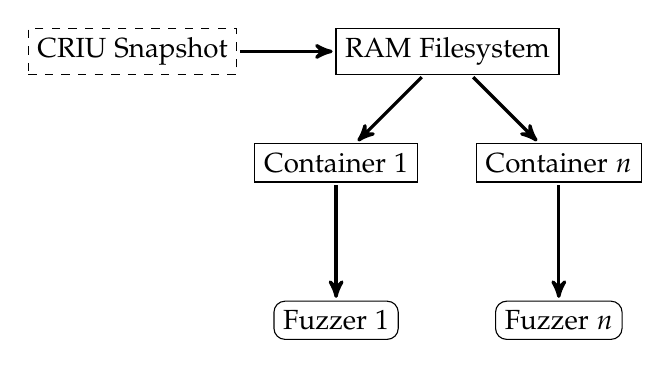
\begin{tikzpicture}[
  node distance=2cm,
  fuzzer/.style={rectangle, draw, text centered, rounded corners},
  container/.style={rectangle, draw, text centered},
  snapshot/.style={rectangle, draw, text centered, dashed},
  arrow/.style={->, >=stealth', shorten >=1pt, shorten <=1pt}
]

% Containers
\node (root) [container] {RAM Filesystem};

% CRIU snapshots
\node (snapshot1) [snapshot, left of=root, xshift=-2cm] {CRIU Snapshot};

\node (container1) [container, below left of=root] {Container 1};
\node (container2) [container, below right of=root] {Container $n$};

% Fuzzers
\node (fuzzer1) [fuzzer, below of=container1] {Fuzzer 1};
\node (fuzzer2) [fuzzer, below of=container2] {Fuzzer $n$};


% Arrows
\draw [arrow, very thick] (root) -- (container1);
\draw [arrow, very thick] (root) -- (container2);
\draw [arrow, very thick] (container1) -- (fuzzer1);
\draw [arrow, very thick] (container2) -- (fuzzer2);
\draw [arrow, very thick] (snapshot1) -- (root);
\end{tikzpicture}
\caption{The CRIU and Docker-based QEMU fuzzing system used to evaluate Jetset's rehosting of emulated systems.}
\label{fig:fuzzing}
\end{figure}

Embedded systems pose a challenge for emulation because their code expects to interact with specialized on-chip and off-chip peripherals, such as general-purpose I/O (GPIO) ports, sensors, and communication interfaces. 
In this dissertation, we consider this specific challenge in the context of \emph{rehosted} emulation.
Introduced in Chapter~\ref{chap:emulation}, rehosting refers to the decoding of information from a system specification into a set of emulated systems capable of executing that system in a different domain, e.g. a laptop computer.
The execution environment must emulate these devices with sufficient fidelity to ensure that observed behavior accurately mimics the target system running on hardware. 
However, because of the large variety of peripheral devices, most are not modeled by the execution environment, creating a considerable blind spot for our most powerful analysis techniques. 
Indeed, there may be no documentation at all about a target system, which makes building a complete emulator for it nearly impossible.

In many cases, however, the code of interest to the system analyst is not the code that interacts with peripherals. 
While peripherals cannot be ignored completely---hardware initialization must appear successful for the system to boot successfully---correct behavior of all devices may not be necessary. 
This chapter will focus on the rehosting approach, which attempts to infer partial but effective models of these missing hardware devices, and Chapter~\ref{chap:integreat} will look at an extraction based approach to this same problem.
For example, an analyst interested in how a target responds to network traffic may not require the execution environment to faithfully model all aspects of the system's GPIO ports or other communication interfaces.

The subject of this chapter is Jetset, a system that performs \textit{targeted rehosting} of firmware\textemdash it automatically infers the expected behavior of embedded system peripherals using only its firmware and then synthesizes a model of the peripherals sufficient to boot to security-critical code of interest. 
The synthesized peripheral model can then be used in an emulator---in our evaluation we used QEMU~\cite{bellard2005qemu}---to emulate the hardware environment. 
An analyst can then use her tool of choice to interact with the firmware. 
For example, a vulnerability analyst can use Jetset to fuzz-test the system to see how it responds to malformed or otherwise malicious input. 
More advanced dynamic analyses, like symbolic execution, are also available to the analyst.

Jetset infers the values that need to be read from peripheral devices needed for the program to reach an analyst-specified \emph{goal address}. 
For example, on the Raspberry Pi target used in our evaluation, our goal is to reach the address where the code jumps to user space. 
Our key insight is that firmware code interacting with a peripheral device implicitly encodes how the device must behave for the system to boot. 
Jetset uses symbolic execution of the firmware---specifically the angr framework~\cite{wang2017angr}---to infer data returned from devices.  

The input to Jetset is the executable firmware image, the firmware entry point (where to start execution), a goal address (the address we want to reach in execution), and a memory layout specifying which parts of the address space represent RAM and which represent memory-mapped I/O. 
Jetset only requires emulation support for the CPU architecture; it does not require any special hardware, and does not use the underlying hardware device.

To evaluate Jetset, we use it to infer and instantiate peripheral devices for thirteen targets: an aircraft Communication Management Unit (AMD 486-based system) used on the Boeing 737, Linux on a Raspberry Pi 2 (ARM-based SoC board), the first-stage bootloader on a BeagleBoard-xM (ARM-based SoC board), a SEL-751 Feeder Protection Relay (Motorola ColdFire-based system), and the 9 publicly available real-world targets from prior comparable work\cite{p2im2020}. 
These targets are diverse\textemdash they come from 3 different architectures, 5 different operating systems (as well as 3 different bare metal systems), and several different application domains.
For each target, Jetset inferred the behavior of its peripherals needed for the firmware to complete its boot sequence,and produced C code suitable for use with QEMU that simulates the inferred devices. 
We then run the firmware in QEMU configured for the target CPU architecture using our synthetic peripherals to complete the configuration.

For two of our targets, we confirm that the synthesized devices work
correctly by comparing the emulated system against a reference.  For
the Raspberry Pi 2, we compare the emulated behavior of the system to its
behavior on actual hardware.  
We used a novel framework capable of snapshotting the QEMU device emulator and instrumenting this with the AFL
fuzzer~\cite{zalewski2017technical} to fuzz-test the Linux
kernel system call interface, obtaining the same results both in QEMU
and on the actual hardware.  For the Communication Management Unit
(CMU), we use a high-fidelity QEMU implementation of the system,
including its most important peripherals for comparison.  We produced
this implementation by manually reverse-engineering the CMU as our
reference. We used our fuzzer to test the system call interface of the
underlying OS on both the reference and synthesized implementations to
confirm we observe the same behavior on both.  Although finding
vulnerabilities was not the goal of this testing, we nevertheless
identified a previously unknown privilege escalation vulnerability in
the VRTX kernel used by the CMU
(Section~\ref{sec:cmu-attack}).
This chapter will also discuss other exploits developed using this emulator analysis and disclosed to UTC aerospace: first, a local code execution method based upon the data loader protocol, and ACARS messages which are capable of disabling a running CMU remotely.

\section{Related Work on Rehosting}
\label{sec:rehost-related}

Due to the complex nature of firmware and the heterogeneity of the hardware it interacts with, security testing and analysis of firmware is a difficult problem~\cite{muench2018you, wright2021challenges}.
Different techniques to test and analyze firmware vary both in their goal (e.g., finding bugs, full rehosting, or partial rehosting), as well as the assumptions that they make about the firmware they analyze.
For example, a testing technique may only analyze firmware using a particular operating system~\cite{firmadyne}, or may assume that auxillary information about the firmware is available (e.g., firmware-hardware I/O traces~\cite{pretender2019}) to improve results.
The use case of Jetset\textemdash partial rehosting using only the firmware itself and no auxillary information\textemdash is most similar to other rehosting techniques, however, for completeness, we outline other approaches to analyzing firmware below.

\paragraph{Firmware testing and analysis}
Approaches have been developed to test firmware without attempting to create a stand-alone emulator for the hardware.

Symdrive~\cite{symdrive} is a symbolic testing framework for Linux device drivers.
Symdrive takes as input the C code for the Linux drivers and attempts to find program paths that violate user written assertions. 
Symdrive is able to uncover numerous bugs in Linux device drivers; however, it requires source code and is Linux specific.

FIE~\cite{fie} is a symbolic execution framework that targets firmware for the
MSP430 family of microprocessors.
FIE takes as input a piece of firmware, a memory map (that denotes which regions are RAM, ROM, MMIO, etc), and an interrupt specification which describes all locations where interrupts could be fired. 
FIE is designed to analyze all firmware execution paths, which, while effective for the simpler MSP430 microcontroller firmware, is not feasible for more complex firmware like the Raspberry Pi's Linux kernel. 
For this complex firmware, a more targeted approach such as Jetset's is needed.
Furthermore, FIE requires the source code for the firmware\textemdash this is how it adds its symbolic execution instrumentation\textemdash and it is therefore unsuitable for our needs.

Revnic~\cite{revnic} is a system for symbolically executing driver firmware and reverse engineering its functionality.
Revnic takes as input a driver binary, a driver template describing the high level functionality of the driver, and domain specific knowledge about the OS of the driver, and produces source code for the driver.
Revnic requires knowledge of the underlying operating system, and requires that the user provide detailed device templates that outline the functionality of the device, and it is therefore unsuitable for the problem of firmware-only emulation.

FirmUSB~\cite{firmusb} is a USB-specific symbolic execution framework for analyzing USB microcontroller firmware. 
FirmUSB takes as input a USB firmware image, and uses domain specific analyses  to identify malicious behavior by the USB device.
For example, FirmUSB can detect if a device claiming to be a USB keyboard is injecting keys that have not been pressed by looking for USB specific information flows.

\paragraph{Hardware-in-the-loop emulation} 
Another method of approaching the problem of analyzing firmware is to attach a software emulator running the firmware to the physical hardware, forwarding I/O between the emulator and the firmware.
Avatar~\cite{avatar} is a dynamic analysis framework for embedded systems that does exactly this.
Other tools 
\textsc{Surrogates}~\cite{surrogates} and \textsc{Prospect}~\cite{kammerstetter2014prospect} build on this hardware-in-the-loop approach.

This technique provides the highest fidelity emulation since the emulator directly interacts with the physical hardware; however, use of this technique is contingent on continuous access to the hardware, which is not always possible since hardware (like that used in avionics) may be difficult or impossible to obtain.

\paragraph{Full firmware rehosting} 
Full rehosting is a technique which attempts to construct a fully featured, high-fidelity emulator from a piece of firmware and auxillary information about the SoC or firmware.

Firmadyne~\cite{firmadyne} is a platform for automated dynamic analysis of Linux-based embedded systems.
Firmadyne takes as input a piece of firmware running the Linux kernel, and executes user-space code for the firmware, emulating the common Linux peripherals.
Similarly, Costin et al.~\cite{costin2014large, costin2016automated} extract and rehost the embedded system's filesystem in their own analysis environment to analyze network-facing code.
Because the code of interest to an embedded system security analyst is often the user-space, network-facing code, Firmadyne and Costin et al.'s tool are well-suited for this scenario. 

Pretender~\cite{pretender2019} rehosts firmware by recording the interactions between the physical hardware and the firmware. 
It then uses a machine learning engine to learn a stateful model for peripheral behavior and creates an emulator from this model.
Similar to Avatar, Pretender takes as input the firmware, and a connection to the physical hardware, and creates an emulation environment; however, unlike Avatar and related tools, Pretender can fully migrate the firmware to a virtualized environment, and does not require persistent access to the hardware.


HALucinator~\cite{clementshalucinator} is a firmware rehosting tool that uses hueristics to locate the code belonging to the hardware abstraction layer (a vendor-provided API for interacting with the hardware) in the firmware and replaces it with manually created handlers. 
HALucinator takes as input firmware, and the HAL the firmware uses, and produces a fully featured emulation environment for the firmware.


Previous rehosting techniques have relied on auxillary information to infer the behavior of the hardware environment.
While this results in a more complete emulator, this auxillary information is not always available\textemdash most of our evaluation subjects had none.
Furthermore, security analysis is often concerned with only a particular software component of the firmware, (e.g., the network traffic or the file system code) and may not need a fully featured emulator.

\paragraph{Partial rehosting}
Partial rehosting, as opposed to full rehosting, attempts to create an emulator from the firmware only, with no auxillary information about the peripherals.
However, the emulators produced by partial rehosting are not complete\textemdash they are not guaranteed to implement all peripherals for the firmware, only what they can infer.
This is the point in the design space that Jetset occupies.
There is one other notable system that implements partial rehosting, P\textsuperscript{2}IM.

P\textsuperscript{2}IM~\cite{p2im2020} does both fuzzing and partial rehosting based on the peripheral model that it infers from the fuzzing stage.
It takes as input the target firmware and its memory map, and fuzzes the firmware code by channeling input from an off-the-shelf fuzzer like AFL to the peripherals. 
It then analyzes the device access patterns exercised during this fuzzing pass to infer details about the memory-mapped IO interactions between the firmware and peripheral devices, and executes the firmware without crashing.

There are two key differences between P\textsuperscript{2}IM's fuzzing-based approach, and Jetset's directed symbolic execution-based approach.
The first deifference is that unlike P\textsuperscript{2}IM, Jetset is \textit{targeted}\textemdash it is designed to ignore most paths through the firmware to focus on a particular target piece of code, which allows it boot deep into large pieces of firmware.
While Feng et al. showed P\textsuperscript{2}IM's approach is effective at fuzzing peripheral handling code and emulating microcontroller code, it is not clear whether it scales to larger firmware.
Besides evaluating against all of P\textsuperscript{2}IM's publicly available real-world evaluation subjects, we also evaluated Jetset against four complex pieces of firmware\textemdash one of our evaluation subjects, the Raspberry Pi 2 is 450x LoC of any of P\textsuperscript{2}IM's evaluation subjects.
We attempted to evaluate P\textsuperscript{2}IM on our 4 real-world firmware samples. Unfortunately, the current version of P\textsuperscript{2}IM only supports Cortex-M MCUs and we were unable to run it on any of our samples, including our Cortex-A7 and Cortex-A8 firmware.

The second difference is that, while fuzzing-based approaches are efficient since they use lightweight executions, they can have trouble bypassing complex checks. 
In Section~\ref{sec:jetset-eval}, we provide an example of a complex numerical check that occurred when inferring the behavior of an FPGA in one of our evaluation subjects.
Jetset is able to handle complex numerical checks, because it performs partial rehosting using symbolic execution.

\section{Jetset's Inference of Hardware Semantics}
\label{sec:jetset-eval}

Jetset uses symbolic execution to infer how peripheral devices must respond to reads from the firmware for execution to progress toward the goal address.
It uses this inferred information to deduce and reproduce expected peripheral device functionality to boot firmware in an emulator such as QEMU.
This allows analysts to boot the system in an emulator with only the firmware, and without the target's hardware or support for the peripheral devices in the emulator.
To do this, Jetset requires the following information about the target embedded system (discussed briefly in Chapter~\ref{chap:emulation}).

\begin{itemize}[noitemsep, leftmargin=12pt]
\item The \emph{executable code} of the target, usually read out of program flash or extracted from a firmware update provided by a manufacturer.
\item The \emph{memory layout} of the target, specifying which regions of the address space are mapped to program memory, RAM, and device I/O registers.
This information can be obtained from the datasheet of a single-chip system or from a basic analysis of the executable code. Note that Jetset does \emph{not} need to know which devices are mapped where, only the address range used for memory-mapped I/O.
\item The \emph{entry point address} where execution begins.
This is often specified in the CPU datasheet.
\item The program \emph{goal address} that the analyst wants the program to reach.
For example, this can be the address of a print instruction that reports a successful system boot.
\end{itemize}

To model peripherals, Jetset uses symbolic execution to \emph{infer} expected device behavior, and then the resulting encoding of the device behavior in the constraints returned by symbolic execution is used to \emph{synthesize} a device suitable for use in an emulator (e.g., QEMU).
Secondary to this \emph{peripheral Modeling} phase, Jetset must also adopt a correct \emph{search strategy} to guide symbolic execution, introduced in Chapter~\ref{chap:prelim}.

\subsection{Jetset's Peripheral Modeling}
In its \emph{peripheral inference} stage, Jetset symbolically executes the firmware to infer what values should be returned by reads from device registers in order for execution to reach the firmware's goal address.
In Jetset, input from devices are marked symbolic and tracked through QEMU's emulation by \emph{taint-tracking} all Tiny Code Generator (TCG) operations and a number of QEMU's helper functions.
During execution, all reads from memory-mapped I/O addresses space are therefore symbolic, while the initial contents of flash and memory are concrete.\footnote{Note that this means Jetset \emph{does not} infer flash devices, something which was manually modeled for the emulation during the QEMU exploit generation.}
Each read from a memory-mapped I/O address returns a distinct symbolic variable; that is, two reads from the same address result in two \emph{different} symbolic values.
Jetset stops when an execution path reaches the goal address, resulting in a set of constraints on values read from device registers that lead to this address.

\paragraph{Interrupts}
While executing, the firmware may also require interrupts to be serviced to reach the target.
Jetset therefore periodically injects interrupts during the modeling stage.
For example, the goal address for the Raspberry Pi firmware is in a different kernel thread than the entry point, so a scheduler interrupt is needed to reach the goal.
From Jetset's point of view, this means that it needs to execute an interrupt service routine (ISR) to make progress.
Given infinite compute resources, Jetset could explore every possible interrupt either firing or not after each instruction.
However, this is impractical.
Jetset exploits the fact that well-designed systems are not sensitive to the \emph{exact} timing of interrupts and that ISRs are written to handle spurious interrupts gracefully.
Jetset periodically injects interrupts during symbolic execution, so that each ISR is executed periodically during each execution path.
If the main execution thread happens to be waiting for an ISR to update a variable, Jetset will eventually execute that ISR, and the thread can continue making progress.

\paragraph{Peripheral synthesis}
Once Jetset has reached the target (with or without interrupts), it can create a synthetic peripheral model that can be used in QEMU.
The result of the inference stage is a set of constraints on values read from peripherals needed for the firmware to boot.
Jetset then uses Z3~\cite{zthree}, the default SMT solver used by angr, to find concrete values satisfying these constraints, capturing in the firmware's expected response to device reads during execution.
This allows Jetsetto construct a light-weight, concrete device model, rendering peripheral modeling a one-time cost per device.

This synthesis stage generates an I/O trace model that is sufficient to reach the goal in the emulator.
The synthesized trace is partitioned by I/O address, so there is a separate trace for each memory-mapped I/O address.
When Jetset reaches the end of an I/O trace for a particular address, any subsequent reads return the last value in the trace.
This allows Jetset to continue past the goal address in emulation, but precludes any complex interaction with the device after the trace has ended (see Section~\ref{sec:jetset-limitations}).

The synthesized device injects interrupts in the same way as during peripheral modeling, ensuring that any necessary ISRs are executed in emulation.
Interrupt timing during execution in an emulator does not need to precisely match the timing during peripheral modeling\textemdash if, during emulation, an interrupt is fired one instruction later, this will not make a difference in emulation.

\subsection{Jetset's Search Strategy}

To ensure that Jetset continues to make forward progress towards the goal address during symbolic execution, which by default attempts to explore the all executable paths, Jetset uses a distance function to guide its search.
This distance function is context-sensitive~\cite{directedsymex}: it takes into account that the distance between two instructions in a program can depend on the calling contexts (i.e., the callstack) of the two instructions.
Computing a context-sensitive distance function is more complicated than computing a local distance (i.e., the distance between two instructions in a single function).
Whenever a decision point is encountered, Jetset chooses the shortest path to the goal location, barring a few exceptions, discussed later.

\begin{figure}
\centering
% Adapted from http://www.texample.net/tikz/examples/flexible-flow-chart/
\newcounter{step}
\newcommand*\step{
  \stepcounter{step}%
  \scriptsize
  \arabic{step}.
  \ttfamily
}
\begin{tikzpicture}[
  % Global options.
  >=Stealth,
  node distance=2.5ex,
  every join/.style={norm},
  every label/.style={font=\scriptsize},
  % Flow chart box styles.
  base/.style={font=\step, draw, on chain, on grid, align=center, minimum height=2ex, inner xsep=.1em, top color=black!10},
  proc/.style={base, rectangle, minimum width=4em},
  test/.style={base, diamond, aspect=2, minimum width=4em},
  % Connector styles.
  norm/.style={shorten >=1pt, ->, font=\scriptsize, pos=.3333},
  % Outline styles.
  outline/.style={draw, rectangle, densely dotted, rounded corners, inner sep=1ex},
]
% CFG for main.
{[start chain=main going below]
  \node[proc]                {call foo};
  \node[proc, join=by {"2"}] {call bar};
  \node[proc, join=by {"3"}] {call foo};
  \node[proc, join=by {"2"}] {ret};
}
\node[outline, fit=(main-begin) (main-end), label={\texttt{main} ($\mathit{length}=7$)}] {};

% CFG for foo.
{[start chain=foo going below]
  \node[proc, right=3 of main-begin] {mem[0x100] = 1};
  \node[proc, join=by {"1"}]       {eax = 2};
  \node[proc, join=by {"1"}]       {ret};
}
\node[outline, fit=(foo-begin) (foo-end), label={\texttt{foo} ($\mathit{length}=2$)}] {};

% CFG for bar.
{[start chain=bar going below]
  \node[proc, right=3.5 of foo-begin] {ebx = mem[0x200]};
  \node[test, join=by {"1"}]      {ebx == 1};
  {[start branch=then]}
  \node[proc, join=by {"\texttt{false}; 1"}] (cond) {eax = 3};
  {[continue branch=then]
    \node[proc, right=1.75 of cond,
          join=by {rounded corners,
                   to path={-|(\tikztotarget) \tikztonodes},
                   pos=.25,
                   "\texttt{true}; 1"}] {eax = 2};
  }
  \node[on chain] (dummy) {};
  \node[proc,
        join=with cond by {"1"},
        join=with bar/then-end by {
          -,
          rounded corners,
          to path={|- (dummy) \tikztonodes -| (\tikztotarget)},
          "1"}] {ret};
}
\node[outline, fit=(bar-begin) (bar/then-end) (bar-end), label={\texttt{bar} ($\mathit{length}=3$)}] {};
\end{tikzpicture}

% vim: set sw=2 sts=2 ts=8 et tw=0:

\caption{Context-sensitive distance from statement 5 (in first \texttt{foo} call) to statement 7 (of second \texttt{foo} call).}
\label{fig:jetset-distance-func}
\end{figure}

The local distance between two instructions is simply the graph distance between the two instructions in the control flow graph.
For example, in Figure~\ref{fig:jetset-distance-func}, the distance from statement 5 to statement 7 (both within \texttt{foo}) is 2.
When computing local distances, the edges for call instructions need to be weighted based on the called function's \textit{length}\textemdash the distance between the start of the called function and the nearest return of that function.
For example, in Figure~\ref{fig:jetset-distance-func}, the distance from statement 1 to statement 4 is not 3, but 7.
This is because, when executing a call instruction, it is not really one instruction being executed, but every instruction until the call returns.
This is further complicated, because the called function may itself call other functions.
Therefore, to compute local distances for each function, Jetset first creates a callgraph of all functions in the firmware, then computes local distances for functions in topographical order.
This ensures that when Jetset computes local distances for a function, it has already computed local distances for every function that function calls.
But this still only gives local distances\textemdash it does not provide distances between instructions in different functions.

Computing the distances between instructions in different functions is more complicated, because functions are often called in more than one context and Jetset is only interested in \textit{realizable paths}\textemdash paths which follow a valid call-return sequence.
For example, in Figure~\ref{fig:jetset-distance-func}, the distance between statement 5 (in \texttt{foo}) and statement 4 (in \texttt{main}) depends on \texttt{foo}'s calling context: if \texttt{foo} was called from statement 1, then the distance is 7, if \texttt{foo} was called from statement 3, then the distance is 2.

Jetset uses a context-sensitive distance function: it determines the distance between an instruction in one calling context\textemdash a (pc, callstack) pair\textemdash to another instruction, in another calling context.
To compute this distance function, Jetset first precomputes local distances for all functions.
Then, Jetset computes the distances between instructions in different functions.
To do this, Jetset takes advantage of the fact that all paths between instructions can be broken up into a sequence of returns, followed by a sequence of calls~\cite{directedsymex} (there will never be an interleaved call and return, because then that would be a local distance!).
Nonlocal distances can therefore be seperated into two distances: the \textit{callstack distance}\textemdash the distance along the sequence of returns up the callstack\textemdash and the \textit{callchain distance}\textemdash the distance along the sequence of calls that lead to the goal address (or the goal address in a specific calling context).

Jetset precomputes all local distances, but both the callstack and callchain distances are computed lazily from the actual stack during execution (it is infeasible to precompute all callstack and callchain distances).
Jetset computes the total context-sensitive distance as the sum of the callstack and callchain distances.

The callstack distance measures the distance from an instruction in one calling context to an instruction that can be reached by a sequence of returns (i.e., instructions in functions in the current callstack).
To compute the callstack distance, Jetset first computes the local distance to the location of the closest \texttt{return} instruction.
It continues summing the distances to each return of each function recursively up the call stack.
It stops once it reaches a function that can reach the target with a set of calls (i.e., a function that is in the target's callstack):

\begin{lstlisting}[language=python]
# Calculate callstack distance
while function not in target_callstack:
  distance += local_distance(cur, ret)
  cur = function.returns_to
  function = stack.next_function  
\end{lstlisting}

For example, suppose Jetset wanted to reach statement 7 (in the second \texttt{foo} call) from statement 5 (in the first \texttt{foo} call).
The call stack distance would be 2, as that is the distance to exit from \texttt{foo} to \texttt{main}, at which point statement 7 can be reached by a set of calls.

The callchain distance measures the distance from an instruction in one calling context to an instruction that can be reached by a sequence of calls.
To compute the callchain distance, Jetset first computes the local distance to the nearest \texttt{call} instruction that leads to the target.
It then recursively sums the distance to each function call on the way to the target:

\begin{lstlisting}[language=python]
# Calculate callchain distance
while function != target_function:
  call = target_callstack.closest_call
  distance += local_distance(cur, call)
  function = call.target
  cur = function.entry     
\end{lstlisting}

Suppose again  that Jetset wanted to reach statement 7 (in the second \texttt{foo} call) from statement 5 (in the first \texttt{foo} call).
The call chain distance would be 5: 3 to reach the second \texttt{foo} call and 2 to descend into the \texttt{foo} call to reach statement 7.

\paragraph{Search Exceptions}
However, there are many cases where due to incomplete semantic modeling and software control flow complexity, jetset is not able to identify a correct path to the current goal address using the context-sensitive CFG.
For example, to cope with loops where taking the shortest path will lead to a hanging state, we \emph{alternate} decisions, to avoid taking the same branch twice where unnecessary.
For these cases, Jetset relies on using the local distance to the nearest return as a fallback distance function.
The incremental CFG generation improves the quality of the CFG over time, so eventually the CFG will contain a path to the target.

Jetset's search algorithm may also guide it to a point in the program where it becomes infeasible to reach the target and it needs to terminate the current path and backtrack to a previous state.
There are two different cases where this occurs.
The first case where Jetset backtracks is when a system reset occurs; it is unlikely that a system reset takes place in a correct boot sequence, and backtracking on system resets allows Jetset to avoid boot loops.
The second case where Jetset backtracks is when Jetset enters a statically-detectable infinite loop.
It is also possible to set explicit ``avoid'' locations which will force Jetset to backtrack if some set of constraints are satisfied.

\section{Evaluating Jetset's Targeted Rehosting}

% Targets Data
\newcommand\mmio{MMIO\xspace}
\newcommand\rpitwo{Raspberry Pi 2\xspace}
\newcommand\cmutarg{CMU-900\xspace}
\newcommand\seltarg{SEL-751\xspace}

\newcommand\comma[1]{\num[group-separator={,}]{#1}}

\newcommand\rpiInfWallClockTime{6m43s}
\newcommand\rpiInfBlocksInCode{238,792}
\newcommand\rpiInfRawTotalBlocks{81194393}
\newcommand\rpiInfTotalBlocks{\num[group-separator={,}]{\rpiInfRawTotalBlocks}}
\newcommand\rpiInfTotalBlocksOnPath{81,194,393}
\newcommand\rpiInfUniqueBlocks{43,157}
\newcommand\rpiInfUniqueBlocksOnPath{43,157}
\newcommand\rpiInfWritesOnPath{84,060}
\newcommand\rpiInfReadsOnPath{83,857}
\newcommand\rpiInfWriteAddressesOnPath{40}
\newcommand\rpiInfReadAddressesOnPath{37}
\newcommand\rpiInfDevicesAccessed{6}


\newcommand\rpiSynthWallClockTime{3.16s}
\newcommand\rpiSynthSymbolicVars{1,384}
\newcommand\rpiSynthTotalConstraints{5,226}
\newcommand\rpiSynthAvgConstraints{3.78}
\newcommand\rpiSynthMedConstraints{4}
\newcommand\rpiSynthMaxConstraints{30}
\newcommand\rpiSynthAvgTraceLen{37.4}
\newcommand\rpiSynthMedTraceLen{1}
\newcommand\rpiSynthMaxTraceLen{1076}


\newcommand\rpiEmuWallClockTime{8s}

\newcommand\rpiEmuRawTotalBlocks{81454594}
\newcommand\printpercent[2]{\FPeval\result{round(#1*100/#2,1)}\result\%}
\newcommand\printpercentmore[2]{\FPeval\result{round(#1/#2-1,1)}\result\%}
\newcommand\rpiRawEmuTotalBlocks{43227}
\newcommand\rpiEmuTotalBlocks{\num[group-separator={,}]{\rpiEmuRawTotalBlocks}}
\newcommand\rpiEmuPercBlocksMore{\printpercentmore{\rpiEmuRawTotalBlocks}{\rpiInfRawTotalBlocks}}

\newcommand\rpiEmuUniqueBlocks{43,255}
\newcommand\rpiEmuWritesOnPath{83,915}
\newcommand\rpiEmuReadsFromTrace{83,857}
\newcommand\rpiEmuReadsBeyondTrace{0}
\newcommand\rpiEmuWriteAddresses{43}
\newcommand\rpiEmuReadAddresses{27}
\newcommand\rpiEmuDevicesAccessed{6}
                                                                           
\newcommand\bbxmInfWallClockTime{5m15s}
\newcommand\bbxmInfBlocksInCode{872}
\newcommand\bbxmInfTotalBlocks{20,198,824}
\newcommand\bbxmInfTotalBlocksOnPath{20,198,824}
\newcommand\bbxmInfUniqueBlocks{484}
\newcommand\bbxmInfUniqueBlocksOnPath{484}
\newcommand\bbxmInfWritesOnPath{938}
\newcommand\bbxmInfReadsOnPath{3,633}
\newcommand\bbxmInfWriteAddressesOnPath{244}
\newcommand\bbxmInfReadAddressesOnPath{61}
\newcommand\bbxmInfDevicesAccessed{11}


\newcommand\bbxmSynthWallClockTime{5.64s}
\newcommand\bbxmSynthSymbolicVars{\bbxmInfReadsOnPath}
\newcommand\bbxmSynthTotalConstraints{8,353}
\newcommand\bbxmSynthAvgConstraints{2.30}
\newcommand\bbxmSynthMedConstraints{2}
\newcommand\bbxmSynthMaxConstraints{74}
\newcommand\bbxmSynthAvgTraceLen{59.56}
\newcommand\bbxmSynthMedTraceLen{3}
\newcommand\bbxmSynthMaxTraceLen{2,770}

\newcommand\bbxmEmuWallClockTime{101ms}
\newcommand\bbxmEmuTotalBlocks{20,198,656}
\newcommand\bbxmEmuUniqueBlocks{483}
\newcommand\bbxmEmuWritesOnPath{938}
\newcommand\bbxmEmuReadsFromTrace{3,633}
\newcommand\bbxmEmuReadsBeyondTrace{0}
\newcommand\bbxmEmuWriteAddresses{244}
\newcommand\bbxmEmuReadAddresses{61}
\newcommand\bbxmEmuDevicesAccessed{11}
                                                                           
\newcommand\cmuInfWallClockTime{5m20s}
\newcommand\cmuInfBlocksInCode{55,016}
\newcommand\cmuInfTotalBlocks{53,143,508}
\newcommand\cmuInfRawTotalBlocksOnPath{27517932}
\newcommand\cmuInfTotalBlocksOnPath{\num[group-separator={,}]{\cmuInfRawTotalBlocksOnPath}}
\newcommand\cmuInfUniqueBlocks{776}
\newcommand\cmuInfUniqueBlocksOnPath{731}
\newcommand\cmuInfWritesOnPath{1,308}
\newcommand\cmuInfReadsOnPath{242}
\newcommand\cmuInfWriteAddressesOnPath{13}
\newcommand\cmuInfReadAddressesOnPath{5}
\newcommand\cmuInfDevicesAccessed{5}


\newcommand\cmuSynthWallClockTime{0.018s}
\newcommand\cmuSynthSymbolicVars{\cmuInfReadsOnPath}
\newcommand\cmuSynthTotalConstraints{756}
\newcommand\cmuSynthAvgConstraints{3.12}
\newcommand\cmuSynthMedConstraints{3}
\newcommand\cmuSynthMaxConstraints{11}
\newcommand\cmuSynthAvgTraceLen{48.4}
\newcommand\cmuSynthMedTraceLen{5}
\newcommand\cmuSynthMaxTraceLen{215}

\newcommand\cmuEmuWallClockTime{289ms}
\newcommand\cmuEmuRawTotalBlocks{27519080}
\newcommand\cmuEmuTotalBlocks{\num[group-separator={,}]{\cmuEmuRawTotalBlocks}}
\newcommand\cmuEmuUniqueBlocks{731}
\newcommand\cmuEmuWritesOnPath{1,882}
\newcommand\cmuEmuReadsFromTrace{242}
\newcommand\cmuEmuReadsBeyondTrace{0}
\newcommand\cmuEmuWriteAddresses{13}
\newcommand\cmuEmuReadAddresses{5}
\newcommand\cmuEmuDevicesAccessed{5}
                                                                           
\newcommand\selInfWallClockTime{2h34m51s}
\newcommand\selInfBlocksInCode{141,750}
\newcommand\selInfTotalBlocks{3,351,484,857}
\newcommand\selInfTotalBlocksOnPath{3,351,484,857}
\newcommand\selInfUniqueBlocks{11,364}
\newcommand\selInfUniqueBlocksOnPath{11,364}
\newcommand\selInfWritesOnPath{32,480}
\newcommand\selInfReadsOnPath{704}
\newcommand\selInfWriteAddressesOnPath{68}
\newcommand\selInfReadAddressesOnPath{26}
\newcommand\selInfDevicesAccessed{5}


\newcommand\selSynthWallClockTime{5.61s}
\newcommand\selSynthSymbolicVars{\selInfReadsOnPath}
\newcommand\selSynthTotalConstraints{11,142}
\newcommand\selSynthAvgConstraints{15.83}
\newcommand\selSynthMedConstraints{5}
\newcommand\selSynthMaxConstraints{1279}
\newcommand\selSynthAvgTraceLen{27.08}
\newcommand\selSynthMedTraceLen{2}
\newcommand\selSynthMaxTraceLen{343}

\newcommand\selEmuWallClockTime{1m1s}
\newcommand\selEmuTotalBlocks{3,351,502,947}
\newcommand\selEmuUniqueBlocks{11,364}
\newcommand\selEmuWritesOnPath{32,480}
\newcommand\selEmuReadsFromTrace{704}
\newcommand\selEmuReadsBeyondTrace{0}
\newcommand\selEmuWriteAddresses{68}
\newcommand\selEmuReadAddresses{26}
\newcommand\selEmuDevicesAccessed{5}

% Misc
\newcommand\numCmuVulns{1}
\newcommand\dtbFileDevices{28}
\newcommand\rpiDistinctSyscalls{1,571,576}

\newcommand\numXloadRegns{200}
\newcommand\numXloadSynDevs{TODO}
\newcommand\numHrsXload{TODO}
\newcommand\numLinxBrch{TODO}
\newcommand\numLinxIndrJumps{TODO}

% RPI Eval Data
\newcommand\rpiSyscallsIssued{}
\newcommand\rpiRawNumPathsDiscovered{123198}
\newcommand\rpiNumPathsDiscovered{\num[group-separator={,}]{\rpiRawNumPathsDiscovered}}
\newcommand\rpiHexDumpDiffsNum{51,592}
\newcommand\rpiHexDumpDiffsPerc{41.9\%}
\newcommand\rpiRawNumDeaths{51638}
\newcommand\rpiNumDeaths{\num[group-separator={,}]{\rpiRawNumDeaths}}
\newcommand\subtract[2]{\FPeval\result{round(#1-#2,0)}\comma{\result}}
\newcommand\rpiNumReturns{71560}
\newcommand\rpiPhysicalTestCases{14,661}

% CMU Eval Data
\newcommand\cmuRawNumPathsDiscovered{2963}
\newcommand\cmuNumPathsDiscovered{\comma{\cmuRawNumPathsDiscovered}}
\newcommand\cmuHoursFuzzed{200}
\newcommand\cmuRawExactOutputMatches{2884}
\newcommand\cmuExactOutputMatches{\comma{\cmuRawExactOutputMatches}}
\newcommand\cmuNearExactOutputMatches{36}
\newcommand\cmuNonExactOutputMatches{43}
\newcommand\cmuDifferenceInBlocksExecuted{\subtract{\cmuEmuRawTotalBlocks}{\cmuInfRawTotalBlocksOnPath}}

\newcommand\cmuPercentNonExactOutputToPaths{1.5\%}
\newcommand\cmuPercentNearOutputToPaths{1.2\%}
\newcommand\cmuPercentExactOutputToPaths{97.3\%}

\newcommand\bbxmDatasheetPeris{35}

\begin{table*}
\centering
\caption{Jetset's primary targets and summary statistics regarding peripheral modeling.}
\label{tab:targets}
\begin{tabular}{@{}lllrrrr@{}}
  \toprule
  \quad                       &                                                     & \multicolumn{2}{r}{\textbf{RPi2}} & \textbf{BBXM}      & \textbf{CMU-900}            & \textbf{SEL-751}            \\
  \midrule
  \multicolumn{2}{@{}l}{OS/SW}   & \multicolumn{2}{r}{Linux 4.19.y}                 & X-Loader                                   & VRTX-32                      & G5.1.5.0                                                  \\
  \multicolumn{3}{@{}l}{\emph{Peripheral inference}}                                                                                                                                                                        \\
                              & \multicolumn{2}{l}{Wall-clock time}                 & \rpiInfWallClockTime                        & \bbxmInfWallClockTime        & \cmuInfWallClockTime        & \selInfWallClockTime        \\
                              & \multicolumn{2}{l}{Blocks in code base}             & \rpiInfBlocksInCode                         & \bbxmInfBlocksInCode         & \cmuInfBlocksInCode         & \selInfBlocksInCode         \\
                              & \multicolumn{2}{l}{Total blocks executed}           & \rpiInfTotalBlocks                          & \bbxmInfTotalBlocks          & \cmuInfTotalBlocks          & \selInfTotalBlocks          \\
                              & \multicolumn{2}{l}{Blocks executed on path}         & \rpiInfTotalBlocksOnPath                    & \bbxmInfTotalBlocksOnPath    & \cmuInfTotalBlocksOnPath    & \selInfTotalBlocksOnPath    \\
                              & \multicolumn{2}{l}{Unique blocks executed}          & \rpiInfUniqueBlocks                         & \bbxmInfUniqueBlocks         & \cmuInfUniqueBlocks         & \selInfUniqueBlocks         \\
                              & \multicolumn{2}{l}{Unique blocks executed on path}  & \rpiInfUniqueBlocksOnPath                   & \bbxmInfUniqueBlocksOnPath   & \cmuInfUniqueBlocksOnPath   & \selInfUniqueBlocksOnPath   \\
                              & \multicolumn{2}{l}{\mmio\ writes (ignored) on path} & \rpiInfWritesOnPath                         & \bbxmInfWritesOnPath         & \cmuInfWritesOnPath         & \selInfWritesOnPath         \\
                              & \multicolumn{2}{l}{\mmio\ reads (symbolic) on path} & \rpiInfReadsOnPath                          & \bbxmInfReadsOnPath          & \cmuInfReadsOnPath          & \selInfReadsOnPath          \\
                              & \multicolumn{2}{l}{\mmio\ write addresses on path}  & \rpiInfWriteAddressesOnPath                 & \bbxmInfWriteAddressesOnPath & \cmuInfWriteAddressesOnPath & \selInfWriteAddressesOnPath \\
                              & \multicolumn{2}{l}{\mmio\ read addresses on path}   & \rpiInfReadAddressesOnPath                  & \bbxmInfReadAddressesOnPath  & \cmuInfReadAddressesOnPath  & \selInfReadAddressesOnPath  \\
                              & \multicolumn{2}{l}{Devices accessed}                & \rpiInfDevicesAccessed                      & \bbxmInfDevicesAccessed      & \cmuInfDevicesAccessed      & \selInfDevicesAccessed      \\
  % Fix to be just the peripherals
  \multicolumn{3}{@{}l}{\emph{Peripheral synthesis}}                                                                                                                                                                            \\
                              & \multicolumn{2}{l}{Wall-clock time}                 & \rpiSynthWallClockTime                      & \bbxmSynthWallClockTime      & \cmuSynthWallClockTime      & \selSynthWallClockTime      \\
                              & \multicolumn{2}{l}{Total Symbolic Variables}        & \rpiSynthSymbolicVars                       & \bbxmSynthSymbolicVars       & \cmuSynthSymbolicVars       & \selSynthSymbolicVars       \\
                              & \multicolumn{2}{l}{Total Constraints}               & \rpiSynthTotalConstraints                   & \bbxmSynthTotalConstraints   & \cmuSynthTotalConstraints   & \selSynthTotalConstraints   \\
                              & \multicolumn{2}{l}{Constraints per variable}   & \rpiSynthAvgConstraints                     & \bbxmSynthAvgConstraints     & \cmuSynthAvgConstraints     & \selSynthAvgConstraints     \\
%                              & \multicolumn{2}{l}{Med. constraints per variable}   & \rpiSynthMedConstraints                     & \bbxmSynthMedConstraints     & \cmuSynthMedConstraints     & \selSynthMedConstraints     \\
%                              & \multicolumn{2}{l}{Max. constraints per variable}   & \rpiSynthMaxConstraints                     & \bbxmSynthMaxConstraints     & \cmuSynthMaxConstraints     & \selSynthMaxConstraints     \\
                              & \multicolumn{2}{l}{Average trace length}               & \rpiSynthAvgTraceLen                        & \bbxmSynthAvgTraceLen        & \cmuSynthAvgTraceLen        & \selSynthAvgTraceLen        \\
                              & \multicolumn{2}{l}{Median trace length}               & \rpiSynthMedTraceLen                        & \bbxmSynthMedTraceLen        & \cmuSynthMedTraceLen        & \selSynthMedTraceLen        \\
                              & \multicolumn{2}{l}{Maximum trace length}               & \rpiSynthMaxTraceLen                        & \bbxmSynthMaxTraceLen        & \cmuSynthMaxTraceLen        & \selSynthMaxTraceLen        \\
  \multicolumn{3}{@{}l}{\emph{Emulator execution to goal}}                                                                                                                                                                      \\
                              & \multicolumn{2}{l}{Wall-clock time}                 & \rpiEmuWallClockTime                        & \bbxmEmuWallClockTime        & \cmuEmuWallClockTime        & \selEmuWallClockTime        \\
                              & \multicolumn{2}{l}{Total blocks executed}           & \rpiEmuTotalBlocks                          & \bbxmEmuTotalBlocks          & \cmuEmuTotalBlocks          & \selEmuTotalBlocks          \\
                              & \multicolumn{2}{l}{Unique blocks executed}          & \rpiEmuUniqueBlocks                         & \bbxmEmuUniqueBlocks         & \cmuEmuUniqueBlocks         & \selEmuUniqueBlocks         \\
                              & \multicolumn{2}{l}{\mmio\ writes (ignored)}         & \rpiEmuWritesOnPath                         & \bbxmEmuWritesOnPath         & \cmuEmuWritesOnPath         & \selEmuWritesOnPath         \\
                              & \multicolumn{2}{l}{\mmio\ reads}                    & \rpiEmuReadsFromTrace                       & \bbxmEmuReadsFromTrace       & \cmuEmuReadsFromTrace       & \selEmuReadsFromTrace       \\
                              & \multicolumn{2}{l}{\mmio\ write addresses}          & \rpiEmuWriteAddresses                       & \bbxmEmuWriteAddresses       & \cmuEmuWriteAddresses       & \selEmuWriteAddresses       \\
                              & \multicolumn{2}{l}{\mmio\ read addresses}           & \rpiEmuReadAddresses                        & \bbxmEmuReadAddresses        & \cmuEmuReadAddresses        & \selEmuReadAddresses        \\
                              & \multicolumn{2}{l}{Devices accessed}                & \rpiEmuDevicesAccessed                      & \bbxmEmuDevicesAccessed      & \cmuEmuDevicesAccessed      & \selEmuDevicesAccessed      \\
  \bottomrule
\end{tabular}

\end{table*}

Jetset's evaluation was dependent upon getting several firmware images into a steady state emulation, where the emulator would run without crashing.
The core targets for this evaluation were a Raspberry Pi 2, a single-board computer based on the Broadcom BCM2836 system-on-a-chip (SoC); a BeagleBoard-xM, a hobbist board, based on the Texas Instruments DM3730 SoC~\cite{bbxm-srm}; a Collins Aerospace CMU-900, an electronic system used on many Boeing 737 aircraft, responsible for handling digital communications between the aircraft and ground stations with an AMD Am486, Intel 486-compatible processor; and a Schweitzer Engineering Laboratories SEL-751 feeder protection relay, used to protect power grid systems, leveraging a MCF54455, a 32-bit microprocessor implementing the ColdFire ISA.
The statistics on the emulation of these systems are given in Table~\ref{tab:targets}.

Details on the emulated and symbolically executed versions of the execution are given by the top and bottom portions of the table. 
Differences, in generally, are explanable due to the backtracking of symbolic execution when it hits an infinite loop (in these cases Jetset must re-execute code and take a different path), and due to slower inference-stage execution.
In the case of the Raspberry Pi, this led to an SD host controller command timeout, resulting in an error message and a register dump. 
During emulated execution with synthetic devices, the SD host controller initializes without a command timeout, thus, the executed blocks counts differ; however, the resulting emulation is resilient. 

We also evaluated Jetset on the nine publicly-available real-world pieces of firmware used to evaluate P\textsuperscript{2}IM\cite{p2im2020}, and all of these rehostings were trivially successful.
In general, the firmware images were non-complex and not symbol-stripped, making their analysis straightforward.
The P\textsuperscript{2}IM used four different ARM SOCs, two Cortex M-3 (STM32F103RB and
SAM3X8E), and two Cortex M-4 (STM32F429ZI and MK64FN1M0VLL12) CPUs.
Five of these systems used Arduino as their operating system, one used the RIOT operating system, and three operated on bare metal.

\subsection{Full Hardware System Emulation Fuzzing}

The useful application of the emulations generated by Jetset required both the development of systems for \emph{fuzzing} and \emph{live binary rewriting} (in the case of the CMU.
For this purpose, we reduced the requirment firmware modification imposed by the FirmAFL~\cite{zheng2019firm} QEMU-AFL combined fuzzer.
A simplified depiction of our final architecture is given in Fig.~\ref{fig:fuzzing}.

We isolated each fuzzer instance into an system-resource isolated Docker~\cite{docker2020docker} container, and then shared a file system folder between these instances.
Docker was used to maintain isolation in the process tree and shared locks / backing files used by the QEMU emulation of the target systems.
Within each fuzzer instance, file system folders were instantated to maintain the initial state of the emulated system, including backing files for flash memory and other peripheral devices, and an installation of QEMU and AFL with either a ground-truth implementation of the system emulation or a Jetset-generated emulation.
For speed, these backing files were mounted into a RAM filesystem, rather than disk, and each container was pinned to one of 32 CPUs.
In order to provide the initial state for QEMU, a Checkpoint-and-Restore in Userspace (CRIU) snapshot was used~\cite{venkatesh2019fast}.
Inside each container, the QEMU instance was run, reading inputs from AFL and writing outputs to the shared folder.
QEMU was instrumented with hooks which would introspect the guest system for crashes or hangs and then signal to the host AFL instance within the container to reset the entire QEMU process tree from a snapshot.
Because the process tree was reset rather than a single process, peripheral models and coprocessors running in separate child processes would also be reset, simplifying the maintenance of state.

The two targets of our dynamic analysis using this fuzzing framework were the Raspberry Pi and the CMU-900.
Both fuzzing sessions targeted the OS system call boundaries of Linux and VRTX, respectively.
While no novel vulnerabilities were found in Linux, all recovered fuzzing outputs were equivalent between the emulateed and physical versions of the Raspberry Pi.
The CMU-900, however, had significantly more successful results.
The AFL fuzzer found 2963 unique code paths during 200 hours of fuzzing, over 200 of which resulted in meaningful crashes.
One of these code paths, crashing on a function return, was bootstrapped into a privilege escalation vulnerability using a ROP chain by the author.
We next discuss the specific results of fuzzing each of these devices.

\paragraph{RPi Fuzzing}

Because the Linux kernel is used widely, we did not expect our testing to identify new vulnerabilities in its system call interface. Instead, our goal was to determine whether our synthesized configuration \emph{behaves the same way:} for all three implementations, we monitored the response of the Linux kernel to each system call and recorded which of the following four observable behaviors resulted:

\begin{itemize}[itemsep=0pt, leftmargin=18pt]
\item \textbf{Kernel ``oops'' or panic.} Both indicate a kernel fault, pointing to a potentially exploitable bug. A kernel ``oops'' does not halt the system, while a panic does.
\item \textbf{Process killed.} The kernel kills the process issuing the system call. In our configuration, the only process is the init process, leading to a kernel panic with a unique error message. Under normal circumstances process death would not result in a panic.
\item \textbf{System call return.} The kernel returns to the calling process. We recover any set errno and return values.
\end{itemize}

In our experiment, we issued \rpiDistinctSyscalls\ distinct system calls from our init process stub to the Linux kernel running in QEMU with our synthetic devices, resulting in \rpiNumPathsDiscovered\ unique codepaths. Of these, none resulted in a kernel ``oops'' or kernel panic. \rpiNumDeaths\ resulted in the kernel killing the init process, and \rpiNumReturns\ in the system call returning to our user process. 
We then carried out the same experiment (using the same exact system calls) using the official QEMU \rpitwo\ configuration with manually-implemented devices.
In all \rpiNumPathsDiscovered\ cases, we observed the same behavior in both the synthetic and manually-implemented configurations, down to fuzzing paths discovered, error stack traces, \texttt{errno} values, and system call return values.

To compare our (synthetic) implementation against the real hardware, we selected a random sample of \rpiPhysicalTestCases\ test cases.
We then booted the \rpitwo\ kernel on the target board and used a custom init process to read system call parameters from a serial port, issue the system call, wait three seconds, and then reboot the system.
Using this interface, we issued \rpiPhysicalTestCases\ system calls on the target hardware.
If the system call returned, our init process printed \texttt{errno} and the return value to the serial console.
Otherwise, we relied on kernel serial console output to determine whether the init process was killed or whether the kernel encountered a fault (``oops'' or panic).
We observed the same behavior on the physical hardware as in the emulator with synthetic devices.

\begin{figure}[t]
\centering
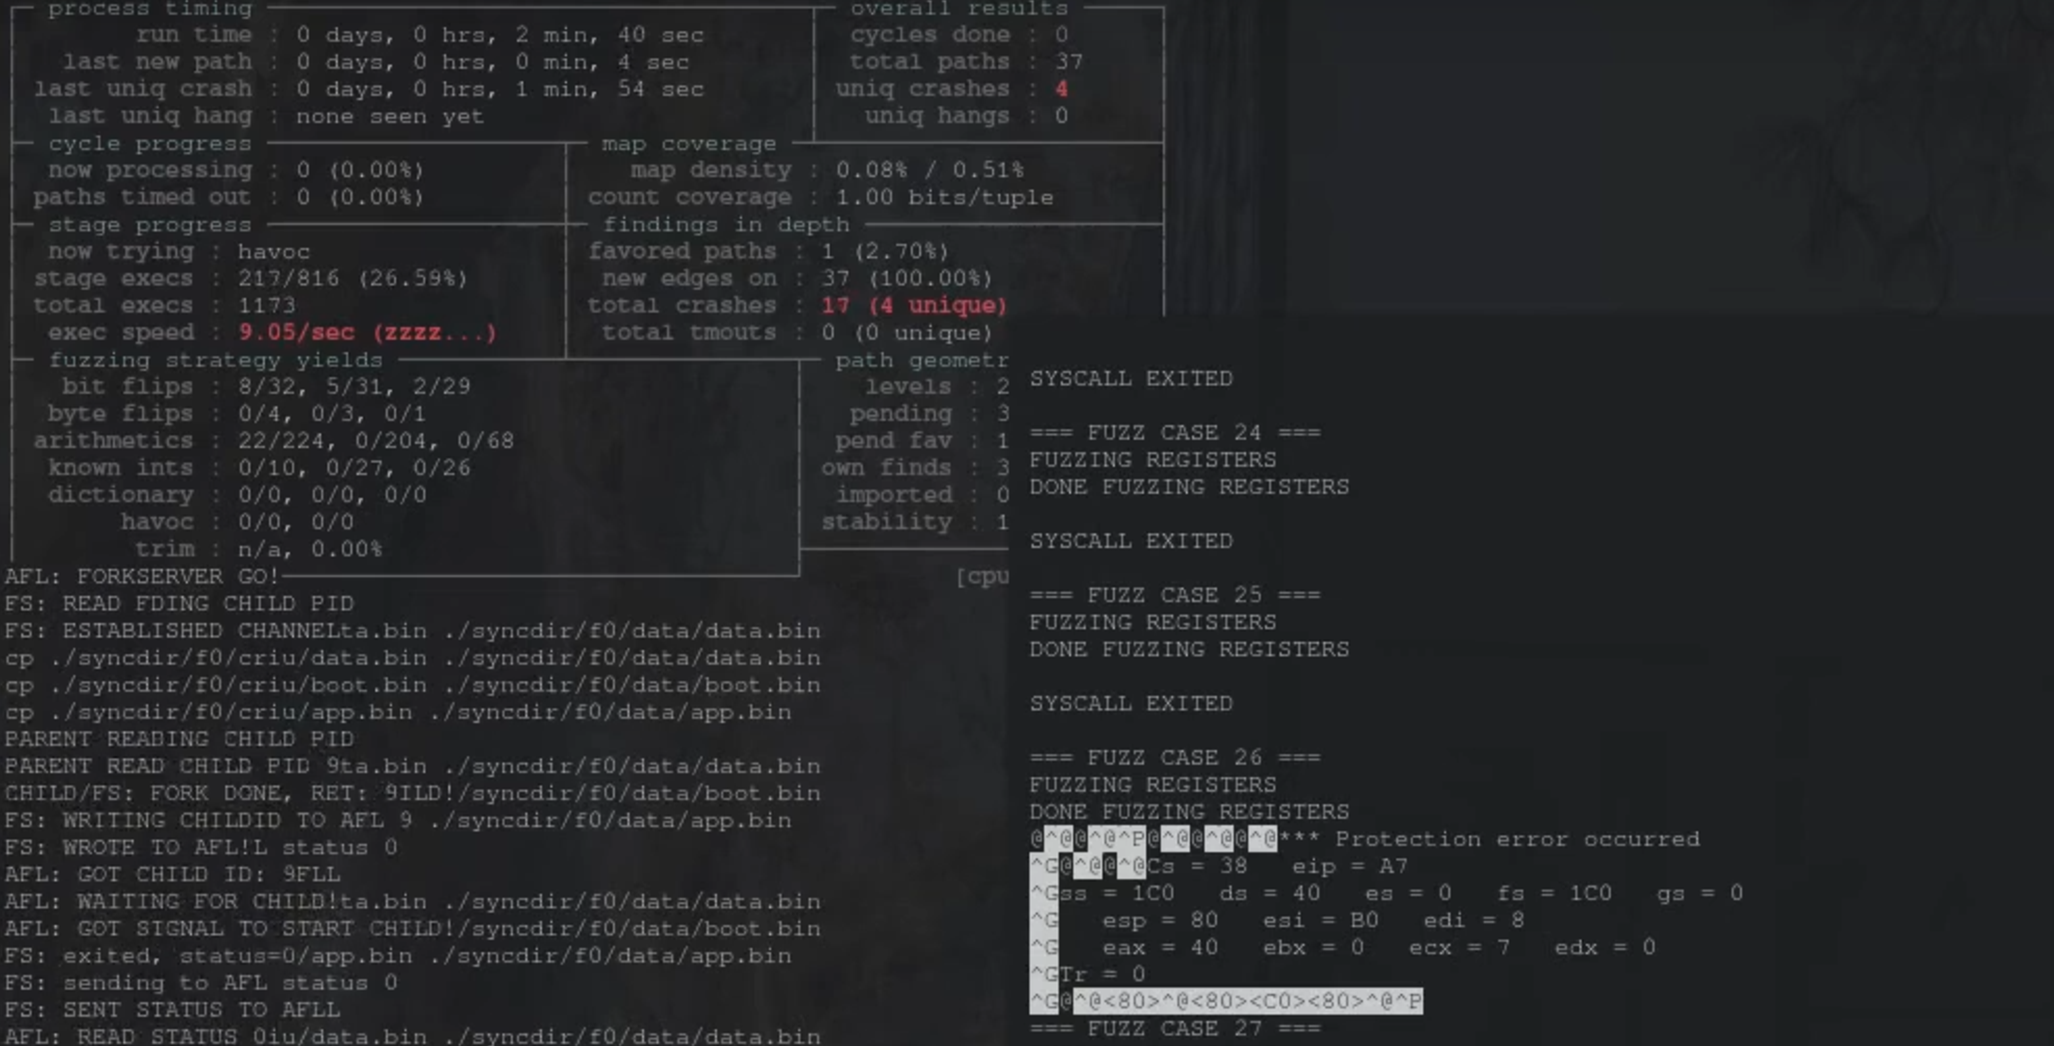
\includegraphics[width=0.9\linewidth]{fuzzing-output}
\caption{A screenshot of the Jetset fuzzing framework (left) discovering a crash (right) in the CMU-900.}
\label{fig:fuzzing-out}
\end{figure}

\paragraph{CMU-900 Fuzzing}
The mainline QEMU distribution implements four of the peripheral devices used by the CMU-900 (the real-time clock, interrupt controller, interval timer, and serial controller).
We created a manual, ground-truth QEMU configuration mapping these devices at addresses expected by the code, which allowed us to compare the behavior of the emulated system with our synthetic devices against a QEMU configured with their full implementation.
As with the Raspberry Pi 2, we compared the behavior of the two systems by issuing system calls from unprivileged task 1.
A screenshot of the fuzzing framework is shown in Figure~\ref{fig:fuzzing-out}.

AFL found \cmuNumPathsDiscovered\ unique crash code paths during \cmuHoursFuzzed\ hours of fuzzing.
To compare the behavior of our two QEMU implementations (synthetic and manual), we compared the debugging console output produced by the \cmutarg.\footnote{
We would prefer to compare the synthetic device QEMU instance to the actual hardware, however, did not want to risk making the device inoperable, one explicit benefit of the emulated copies.
}
In the case of a successful system call return, the \cmutarg\ continues with its normal unprivileged task startup sequence.
In the event of a protection violation, the \cmutarg\ prints a wealth of debugging information, which we use to determine whether the two configurations behaved similarly.

Of the \cmuNumPathsDiscovered\ execution paths discovered by fuzzing, \cmuExactOutputMatches\ (\cmuPercentExactOutputToPaths) \ code paths exhibited identical behavior.
Another \cmuNearExactOutputMatches\ (\cmuPercentNearOutputToPaths) had the same outcome, but differed in the values in some of the registers.
The remaining \cmuNonExactOutputMatches\ (\cmuPercentNonExactOutputToPaths) also had the same outcome, but differed more extensively in the output generated.

Manual analysis of the \cmuNumPathsDiscovered\ execution paths led to
the discovery of a privilege escalation vulnerability.  The
vulnerability occurs because a single byte can be ``leaked'' from
unprivileged code into the offset of a call instruction in the VRTX
kernel.  One of the 256 potential values for this byte results in the
call targeting the middle of a function.  From here, a Return-Oriented
Program (ROP) chain can be used to modify the global descriptor table
(GDT).  A few instructions later, the GDT modification causes the
kernel protection error handler to fire.  However, the GDT
modification changes the base address of the data and stack segment
used by the handler so they overlap with an unprivileged data segment.
The handler includes a far call whose address is dependent upon a read
from the corrupted data segment.  A malicious address can be given to
this far call, leading to a second ROP chain which further modifies
the GDT.  This ROP chain changes the address range limits for
privileged code and transfers control to unprivileged, writable memory
while remaining in processor ring 0.

We were able to validate the exploit on another CMU-900 (one with a slightly different part number and
memory layout) after some minimal adaption and a live binary rewriting process paired with a local code execution exploit which ``poisoned'' the VRTX operating system with shim code. 
Due to small changes in the VRTX kernel between device versions, we discovered
the exploit's control transfer required supplying one ROP gadget address via a
segment rather than a data register and changing some gadget offsets.

\subsection{Leveraging Emulation in Avionics Exploit Development}
\label{sec:jetset-attack}
\label{sec:cmu-attack}

While the loading capability used to introduce software into the physical CMU was provided by the Triton Avionics Testbed~\cite{crow2019triton}, significant additional live binary instrumentation was needed to evaluate the exploit discovered above, and the techniques that were developed in this process allowed us to develop a mechanism for poisoning the CMU-900's VRTX operating system and led us to the discovery of three sets of messages capable of remotely disabling the CMU-900.
Because Aircraft Communication and Reporting System messages also have a ``broadcast'' mode, these messages could be used to crash a large number of CMU-900 devices simultaneously.
Due to their sensitivity, we omit the details of these messages from this dissertation and focus on techniques for their discovery, noting only that one message generates a buffer underflow where memory is allocated beyond the appropriate length and the other two cause excessive memory allocations which drain the availability of new heap memory.

The ability to run the CMU-900's VRTX operating system in an emulated environment was critical to the development and testing of these techniques and associated exploits.
The emulated copies of the CMU-900 allowed us to attempt numerous instrumentation approaches and gain visibility into implementation flaws, a task which would have been significantly more difficult on the physical device.

\paragraph{Bootloader and OS Initialization Replication}
Once our malicious software is loaded into the CMU-900 using the dataloader, control is effectively transferred entirely to the malicious code as a bootloader, negating any prior operating system and hardware device initialization.
It was thus necessary to replicate the bootloader and operating system initialization process in the emulator to ensure that the malicious code would be able to run in the same environment as it would on the physical device.
So, in this initial case, the malicious code would first relocate itself to an unused portion of RAM, transfer control to this new location, replicate the bootloader and initialization behavior necessary to reset the system back to an appropriate initial state, and then return control to to the orginal VRTX operating system.

Developing this replicated functionality required significant manual extraction and analysis of code using Ghidra.
The complexity of dealing with self-relocating code and the specific magic numbers involved for resource initialization led this ``poisoned'' version of the VRTX boot sequence required hundreds of lines of hand-written x86 assembly.
The development of this \emph{in situ} emulation also required significant universal quantification over possible relocation addresses as an alternative to the manual process of identifying a suitable relocation address, a unique benefit of using an emulated system, and served as one inspiration from the redaction attacks presented in Chapter~\ref{chap:info}.

\paragraph{Flash Code Relocation and Shim Injection}
For the purposes of analyzing the system for crashing inputs and testing the system call paths discovered by fuzzing in the previous section, it was not enough to \emph{replicate} the boot process.
Thus, we also performed binary rewriting of operating system code in order to inject instrumentation routines for the purposes of dynamic analysis.

This was complicated by the fact the CMU-900 executed a significant portion of its code out of flash memory, which was considered to be read-only in order to avoid damaging the physical unit.
It was therefore necessary to relocate the portions of code that were to be instrumented into unused, writable RAM memory, and update associated pointers.
This was a two stage process, first consisting of corrupting the interrupt vector table in order analyze portions of the code that were in use at runtime for critical functions and relevant to exploitation, and second, updating non-relative memory addressing data to point to the relocated code segments.

However, once the appropriate relocation operations were complete, it was possible to inject additional shim code at arbitrary locations in system memore using binary rewriting tactics.
The primary rewriting tactic used was the augmentation of x86 call locations, and is detailed in Section~\ref{sec:dynanal} of this dissertation.
With shim instrumentation in place, it was trivial to manually identify potentially crashing inputs by examining data flows within the system.

\section{Open Challenges in Rehosting} 
\label{sec:jetset-limitations}

Returning to the primary subject of Jetset, the approach of targeted rehosting works well for firmware running on a variety of embedded system architectures across multiple application domains. 
However, this approach to peripheral modeling and system emulation is not without limitations, which we break down into \emph{internal} and \emph{external} semantic challenges.

\paragraph{Internal Semantics}
The paths explored by Jetset through firmware are not necessarily ones that may ever be returned by the hardware in the original system; however, the path taken is one that is acceptable to the firmware\textemdash no interaction with any of the peripherals results in a boot failure.
While the execution of firmware running on physical hardware is constrained in its behavior by how the physical peripherals really behave, these system constraints are external to the firmware and cannot be inferred without auxiliary information about its behavior.
To effectively emulate a system, it is not necessary not only to explore a single execution path, but to reveal the connections and meaning implied by multiple execution paths, a topic we will approach in Chapter~\ref{chap:info} and refine in Chapter~\ref{chap:integreat}.

\paragraph{External Semantics}
Jetset does \textit{targeted rehosting} in that it only constructs an emulator that is sufficient to emulate the software component-under-test.
However, rehosting may have no method of deducing the semantics of devices that the system depends upon if the only information it considers is that which is contained within the system specification which remains after these devices are removed, e.g. firmware.
Jetset could be extended to synthesize more complex, stateful peripheral models as well as identify known peripherals with existing emulator implementations using additional information from external sources.

Included in external semantics is the information requires to solve the dynamic analysis challenges presented by Section~\ref{sec:jetset-attack}, which exist outside of the simple execution of a given system model.
While this information is of less general application, it still plays a critical role in quantifying the security of the emulated system, as evidenced by its utility in exploit development.

\section{Summary}

In this chapter, we discussed one approach to the emulation of complex systems, targeted firmware rehosting.
The benefit of this approach is its ability to synthesize peripheral hardware devices for the analysis of real-world embedded systemss.
Particularly, it considers the available information about the system to derive models of unknown components.
In the next chapter, we will develop an alternative approach which addresses some of the shortcomings of looking at a strict derivation from available information for resolving unknown components: universal quantification over possible missing information, and see how this approach applies to the security of real-world redactions.

\chapter{Simulation for Digital Forensics}
\label{chap:info}

\section{Introduction}

\section{Recovering Algorithms}

\section{Redaction Case Study: Shifting Schemes}

\section{Redaction Case Study: Deredaction Attacks}
\label{sec:redaction-attack}

\section{Privacy and Ethics}
\label{sec:redaction-ethics}

\section{Summary}


\chapter{Logic-based Function Extraction}
\label{chap:integreat}

In the approaches to emulation-based measurements of system security we have considered thus far, the primary limitation has been the representation of missing information.
In real-world systems, components are often only partially accessible due to a mixture of closed-source code, limited physical accessibility, or intractable complexity.
Traditionally, the extraction of clean mathematical models from systems, such as ordinary differential equations, is considered infeasible.
Simultaneously, a significant amount of work has now been performed on the verification of models with black-box components, such as DryVR~\cite{fan2017dryvr}.
In this chapter, we will discuss an alternative method of verifying complex, real-world systems which works by extracting key information from a given complex system's binary representation.
We will introduce the InteGreat system~\cite{bland2023integreat}, which uses a combination of a logical rule specification framework, program slicing, and abstract interpretation to lift high-level emulations (continuous equation models which can be dropped into Matlab Simulink).
In the latter sections of this chaper, we will demonstrate how this approach can be used to identify differences between implemented machine code and published mathematical specifications.

\section{Introduction}

Verification of cyber-physical systems (CPS) is a challenging problem, often simplified by the treatment of complex implemented components as black-boxes.
When considering the system itself, mathematical expressions for these systems must often be translated into low-level languages (C, Ladder Logic, etc.) and compiled for use in a physical system.
The resulting binary code may also be symbol-stripped and lose information, e.g. the names of variables, present in the original control algorithm.
In many cases, however, because the system retains something of the high-level semantics, it should still be possible to recover the original high-level model intended for a verification system.
As an added benefit, by working directly with firmware, we could verify and analyze programs where no high-level specification has been written.

While tools such as Ghidra~\cite{eagle2020ghidra} are capable of lifting a binary to pseudo-C representations, these outputs cannot be translated into a more abstract representation of the program.
Adapting these existing tools to lift to a given higher-level representation also requires significant effort, as their internal representations are static and aimed primarily at capturing microarchitectural semantics.
However, if natural deduction could be applied to express the nature of the semantic patterns as they appear in the binary, then lifting to a particular abstract representation could be made modular and portable.
This presents two particular problems of extraction and incorporation: in the former case, the ability to derive an abstract semantic from machine code operations, and the ability to incorporate outside information into the lifting process.

The current state of the art in function extraction involves the use of binary symbolic execution to derive a model of the binary's code over the theory of bitvectors, as was performed in part in Section~\ref{sec:jetset-eval}.
This approach deduces a mathematical model of a computation's behavior, but does not provide any framework for encoding common rules of abstraction.
Moreover, no current binary symbolic execution systems do not provide any means of precisely defining slices of the program to serve as boundaries for the lifting process, and rely on the user to isolate and substitute any subtrees of the AST for simplified expressions.
The result is a set of systems that could theoretically serve to automatically lift a binary to a higher-level representation based upon logical rules, but which in practice lack much of the necessary automation.

We therefore introduce InteGreat, a system which takes in a set of logical lifting rules (provided via Z3~\cite{zthree}) and outputs of symbolic execution to translate closed-source, symbol stripped binary firmware into verifiable mathematical models.
We achieve this by allowing users to nest and chain rules for lifting and decompilation in a natural, declarative syntax, allowing for the modular capture of complex semantic operations.
For example, we may associate a sequences of calls to multiple different child functions as a single operation and we lift a sequence of non-adjacent low level instructions into a single function call using the same effective syntax.
To our knowledge, this is the first lifter to use explicit logical propositions in targeting the correct abstract domain representation of a binary program.

InteGreat significantly extends the angr~\cite{angrsok} symbolic executor to bind the semantics of analyzed program slices into meaningful abstract symbols, replacing complex inner computations with a uniform representations, while maintaining the integrity of the symbolic state's semantics.
In particular, we focus on lifting to continuous equations that may be ``dropped in'' as Matlab Simulink function blocks~\cite{matlab} for evaluation in the context of an environmental model.
Under the system's default operation, a user only needs to specify entry and exit points in the firmware binary, and the system will replace function calls with uninterpreted functions, lifting sequences of otherwise complex operations into a single symbolic value.

To demonstrate the capabilities of such a system, we use InteGreat to show how logical rules can be used to lift continuous equations from a quad-copter firmware implementing Sebastian Madgwick's Orientation Filter~\cite{madgwick, drone}, and demonstrate these lifted equations uncover an implementation error in the quad-copter firmware, finding a three-way difference between the stabilization algorithm's mathematical representation, C, and third-party C implementations.
We also analyze a PLC firmware regulating a chemical plant's reactor pressure~\cite{ICSREF} and use the equations recovered by InteGreat to determine the sensor inputs necessary to precisely destabilize the reactor pressure of the chemical plant and exactly reproduce a code upload attack performed by prior literature.
The lifted representation of the chemical plant's firmware also communicates a subtle discovery: it is not possible to automatically infer representations of analog-to-digital unit conversions at I/O boundaries without additional information from a model of the physical environment.

\section{Related Work on Lifting}

This work brings together multiple methods from a rich history of verification of software and firmware systems.
While our discovery, the application of logics to the domain of decompilation and lifting, is novel, we are indebted to prior work for the introduction of nested abstractions, abstract interpretation, program slicing, function summarization, and many other techniques:

\begin{itemize}
	\item Currie et al.~\cite{currie2006embedded} use the substitution of program slices with uninterpreted functions to determine program equivalence across compiler optimizations.
	However, they do not address the idea of using nested logical rules to perform lift binary programs or the complexities involved in stitching together abstracted program slices.
	We provide a total framework for retaining viable semantics before and after skipping a program slice, even at the bitvector level.
	In fact, Currie et al. note that there may be ways to improve the accuracy of their matching by ``combining uninterpreted functions with a bit of bit-level analysis.''
	\item Sery et. al~\cite{interpolation} leverage the FunFrog system~\cite{sery2012funfrog} to extract function summaries after an initial verification run using source-code level symbolic execution to recover a Bounded Model Checker (BMC) logical formula representing the original program.
	The work performs AST slicing and variable binding methods similar to our own and uses the Craig interpolation (the identification of a sub-proposition that implies two other statements) to refine their function summaries.
	In contrast, InteGreat targets firmware and thus supports the abstraction of micro-architectural semantics.
	We also introduce the idea of using logical formulae to give rules for the translation rather than strict substitution of abstracted program slices based upon the semantics of the slices themselves (interpolation).
	\item A line of work has been done using symbolic execution to perform model extraction and subsequently verification on the extracted models.
	SPIN~\cite{spin}, defined the term ``model extraction'' and applied model-checking on aero-space flight software.
	Babi\'c and Hu~\cite{babic2007structural} used natural abstraction boundary identification and symbolic execution to optimize the performance of verification.
	Hernandez et al.~\cite{firmusb} and~\cite{cryto-symex} used symbolic execution to extract and verify protocol models.
	The same authors also noted the importance of rounding the floating-point precision error on verifying their extracted models in~\cite{precision}.
	Jackson and Woodward~\cite{lightweight-oo} extracted object-oriented (OO) models from Java byte-code,~\cite{oo-model} extracted OO data models from weakly-typed source code. 
	Bandera~\cite{tool-supported-program-abstraction} is a tool for user-guided extraction of finite-state automata from Java programs, however, the tool requires access to source code, and focuses on abstracting single variables rather than program slices.
	While all of these techniques could improve InteGreat, prior work does not address the possibility of a generic framework for the specification of lifting operations, and does not solve the specific problems involved in stitching together uninterpreted functions as abstractions.
	Our work also does not rely on static matching of semantic patterns and supports nested and chained natural deduction rules for lifting.
	\item Ji et al.~\cite{transformation} perform backward application of extended sequent calculus rules on symbolic expression trees.
	Our use of nested logical statements is similar to sequent calculus, however, the goal of Ji et al. was the bisimulation and optimization of the analyzed algorithms using sequent calculus, not to perform lifting.
\end{itemize}

Ultimately, we were somewhat suprised by the lack of a work approaching the subject of extracting functions from a system using logical operations.
However, this use case was also motivated by the specific insights introduced in the emulation and modeling of highly complex systems (Chapters~\ref{chap:rehost} and~\ref{chap:info}).
The InteGreat system draws on the specific challenges of the Jetset and Edact-Ray systems to inform its unique approach to the modeling of systems.

\section{Design of a Logic-based Lifting Specification}

We begin our design of InteGreat with program slices, introduced in Section~\ref{ref:lifting-prelim}, which we denote with $\gamma$, and the location of which we denote $f$.
By default we resolve each $\gamma$ to a function call boundary, but the determination of each $\gamma$'s location is also user-scriptable via a provided wrapper around Ghidra's static analysis APIs.
We enforce that the control flow of each slice must have either a total or no overlap with any other slice (an independence system).

As InteGreat runs, it begins analysis at the innermost $\gamma$ and works outward, identifying all the input and output locations (side effects) of each $\gamma$ via symbolic execution.
By default, these side effects are used to abstract the semantics of each $\gamma$ into a single uninterpreted function mapped to $f$ (the location of the call).
Specifically, we perform three actions upon reaching a location $f$ for a given $\gamma$:
\begin{enumerate}
	\item We associate $f$ to a set of logical formulae for lifting rules
	$\phi$, potentially input by a user, providing a deductive
	sepecification for \emph{how} to lift $f$. For example, encoding the
	logic of splitting a floating point value across r0 and r1.
	\item We associate $f$'s symbolic state with the set of input locations
	of $\gamma$: every potential register and memory location used by the
	output constraints provided by a full symbolic execution of $\gamma$.
	These are then available as symbols in $\phi$ to determine the
	appropriate parameterization of $f$.
	\item We associate encountering $f$ with a specific timestamp to ensure
	the lifted representation respects the program's order of operations.
\end{enumerate}

Our framework provides prospective solutions to the problems of unconstrained pointer values and loop invariant inference during symbolic execution.
To cope with unconstrained pointers we represent each read or write to memory with both the value and the symbolic expression used to determine the address, and enforce a strict equivalence between the two (discussed next).
We expect a zero-length program slice and associated $\phi$ to be defined which can be used to resolve any runtime-ambiguous values of pointers.
For many problematic loops, we can define two program slices: an outer which captures the formulae for handling the loop guard condition and an inner which captures the loop's body expression.
If suitable, we may then replace the guard condition with a concise symbolic represenation, e.g. $\Sigma$, and the inner with an inferred representation of the effects of the loop body as it relates to the outer operation.

As a fallback for fully automatic use of InteGreat, we accept the traditional symbolic execution search strategy of unrolling loops and provide a few sensible defaults for the search strategy, e.g. taking the state that generates the most complex set of constraints or the largest number of writes to memory.

Once the specific challenges of potential state explosion are dealt with, each $\gamma$ is associated to a new symbol $s_{0}, s_{1}, \dots$ and $\phi_{0}, \phi_{1}, \dots$ to perform a translation into a new, higher-level language.
These formulas are also \emph{nestable}, and rules may be written which take some $s$ and $\phi$ as input to produce a second $s'$ and $\phi'$.
For InteGreat's evaluation, we introduce $\phi$ and $\gamma$ such that unmanagable machine code is be abstracted into a Matlab-identical representation inside Z3.
Thus, theorem prover expressions serve as a flexible intermediate representation throughout the lifting process.

\paragraph{Symbolic Memory}
\label{sec:symb-mem-expl}
In most firmware programs, inputs and outputs are context-sensitive to its program state, for example, the dynamic execution stack, or a dereferenced pointer to a memory location.
It is thus necessary for InteGreat to allow symbolic expressions as memory addresses via a $LOC$ function.

InteGreat accomplishes this by implementing a symbolic memory model, extending Trt{\'\i}k et al.'s model~\cite{symbolic-memory}, under-constrained memory~\cite{Under-Constrained}, and incorporating the core ideas of Coppa et al.~\cite{coppa2017rethinking}.
Leveraging the angr event hook infrastructure, InteGreat intercepts all program state modifications, and integrates them with effective address use tracing in order to identify \emph{aliasing}, which occurs when two symbolic pointers are used to reference the same location but their specific value is runtime dependent.
With each pointer dereference, the symbolic memory model is queried with the intercepted dynamic symbolic state of the symbolic executor, which handles returning the correctly intended high-level variable value.

Pointer reasoning is provided by the equivalence of symbolic expressions for pointer values.
When resolving memory, we use timestamps associated with each memory operation and a strict equivalence check on the pointer expression to determine when a memory location is modified.
For example, given two pointers $p_{1}$ and $p_{2}$, if $p_{1} = 50$ and $p_{2} = 50$ at runtime and we are checking $read(p_{1}) = write(p_{2})$, we will return that they are NOT the same memory location. 
That is, we do not assume runtime knowledge. 
We assume that if such knowledge is needed, a zero-size program slice (an entry point address equivalent to the exit address) will be defined that will identify this runtime equivalence, and other tools exist for this~\cite{hind2001pointer}.

\paragraph{Correctness}
Traditional views of compiler (and by extension, decompiler) correctness involve ensuring uncompiled programs, interpreted over an input, result in the same output as compiled programs interpreted over the same input.
In the bottom-down view of compilation from a language operating over $\mathbb{R}$, we already implicitly accept the imprecision introduced by compiler/ISA when equations were compiled are executed.
One argument for the correctness of InteGreat's approach is that we may implicitly accept the imprecision introduced by the inverse operation: lifting from the ISA to the real domain semantics.

However, this does not deal explicitly with the information lost in InteGreat's approach to lifting, as features from the initial domain $\mathbb{D}$ may not be present in $\mathbb{D}'$.
In our earlier example, we mapped from an operation over a Galois field of 64-bit floating point values to an uninterpreted function over $\mathbb{R}$, and the semantics of the Galois field are not preserved in the uninterpreted function.
This trust in the decompiler is further strained when we begin to talk about abstracting arbitrary, complex program slices.
For example, the compiled version of a derivative function may be entirely different in implementation than a Matlab continuous domain equivalent.

We therefore rediscover a common solution to the problem of determining equivalence between complex computations: correctness is ensured by a reduction proof from the original function to the abstract function given a configurable error bound on the difference between outputs in $\mathbb{D}$ and $\mathbb{D}'$, $\varepsilon$.
A similar approach was outlined in Section~\ref{sec:encdec}.
The structure and representation of this proof is flexible and domain-specific, so long as it incorporates $\Phi$ and guarantees the limit $\varepsilon$ holds.
Proofs must be performed on a case-by-case basis as the non-abstracted function and targeted domains can take any of infinite forms.
For example, a proof for a straight-line program performing floating point operations could consider the error introduced by each operational step in the concrete case, and then chain these values together in order to derive a total acceptable bound for $\varepsilon$.
In the present chapter, we forgo a general proof and demonstrate equivalence empirically.

\paragraph{InteGreat's Interface}

\emph{Sufficient input to InteGreat is a program binary, an entry point at which to begin symbolic execution and a list of start and end addresses of program slices.} 
Slices $\gamma$ take the form of a range of addresses (potentially of zero length), a type of instruction, or an expression over the names of other slices.
To avoid repeating the same $\phi$ for multiple $\gamma$ referring to the same operations, we allow multiple range specifications for a given slice.
This input is provided by a series of files which name each $\gamma$ and provide $\Phi$ via a \emph{binds} array of assignments where the left hand side is a symbol name and the right hand side is a Z3 expression.

\emph{Binds} is initialized with the following two symbolic name sets:
\begin{enumerate}
	\item The inferred inputs of $\gamma$, e.g. i0, i1, \dots,
	\item Any prior expressions in the symbolic executor's state prior to reaching $\gamma$, and (optionally)
	\item The full \emph{inner} expression sets for $\gamma'$ inside of $\gamma$ before and after the application of the $\phi'$ associated to the specification of $\gamma'$.
\end{enumerate}
(3) is equivalent to preserving in memory the outputs of prior InteGreat lifting steps, allowing us to nest lifting rules in a modular fashion, and (2) allows us to ``chain'' lifting rules such that, given $\gamma'$ following $\gamma$, symbols returned by $\gamma$ can be used to reason about the lifting of returned by $\gamma'$.

The output of InteGreat is a simplified Z3 AST corresponding to the application of the lifting rules. 
In the evaluation of InteGreat, we structured program slices and inference rules such that translating the Z3 AST to Matlab was trivial.
However, the generic structure of Z3 as an intermediate representation makes it suitable for other tasks, e.g. inferring fixed points and loop invariants for lifted code~\cite{si2018learning}.

% All functions are implemented in Python 3.9.

% 2. \emph{Sequent Inference Algorithm} - This algorithm is used to perform sequent inference on the symbolic execution state.
% 3. \emph{Abstraction Resolution Algorithm} - This algorithm is used to perform abstraction resolution on the sequent inference results.
% 4. \emph{Director Algorithm} - This algorithm is used to perform symbolic execution on the merged state.

% Hooks & symbolic memory

\renewcommand{\algorithmicrequire}{\textbf{Input:}}
\renewcommand{\algorithmicensure}{\textbf{Output:}}

\begin{algorithm}
    \caption{Abstraction Lifting}
    \begin{algorithmic}[1]
        \Require $\gamma$, $binds$
        \Ensure $A_{\Phi(P)}^{f}$
	    \State $A_{P}^{f} \leftarrow SE_{\mathbb{D}}(\gamma)$
 	    \For{\textbf{each} i \textbf{in} inputs($A_{P}^{f}$)} \algorithmiccomment{Bind input to expressions}
	    \State $binds_{i} \leftarrow READ(LOC(i))$
        \EndFor
        \For{\textbf{each} o \textbf{in} outputs($A_{P}^{f}$)} \algorithmiccomment{Bind abstract expressions to output}
	
	    \State $E[outputs_{o}] \leftarrow \Phi_{\gamma}(o)$ \algorithmiccomment{Apply deduction rules}
	    \State $v \leftarrow new\_sym\_name()$
	    \State $binds_{v} \leftarrow E[outputs_{o}]$ \algorithmiccomment{Associate name to expression}
	    \State $WRITE(LOC(o), v)$ \algorithmiccomment{Write abstraction to symbolic memory}
        \EndFor

        \For{\textbf{each} b \textbf{in} $binds$}
	    \State $binds_{b} \leftarrow \Phi(b)$\algorithmiccomment{Common axiom support}
        \EndFor
    \end{algorithmic}
    \label{alg:abst-binding}
\end{algorithm}

\paragraph{InteGreat's Algorithm for Lifting}
\label{sec:integreat-alg}
Before describing the InteGreat's lifting algorithm, we introduce some notation.
Let $A_{P}^{f}$ to refer to the AST returned by angr prior to the application of $\Phi$, similar to Def.~\ref{def:nested-summarization}, and $E$ to refer to an intermediate storage location for Z3 AST expressions.
$\Phi_{\gamma}$ refers to the set of logical statements registered for $\gamma$, $\Phi_{\gamma}(o)$ refers to the full set of statements used to derive $o$ in $\Phi$ from the \emph{binds} array.
Recall that we also implement a symbolic memory addressing system for unconstrained pointer values; we represent locations (either in registers or memory) through the $LOC$ function.
Note that $READ$ and $WRITE$ operate on $A_{P}^{f}$ to produce $A_{\Phi(P)}^{f}$.
$SE_{\mathbb{D}}(\gamma)$ refers to an augmented form of symbolic execution of $\gamma$ using angr in the domain $\mathbb{D}$.

Algorithm~\ref{alg:abst-binding} presents InteGreat's core lifting mechanics.
As noted, the input to the algorithm is a program slice $\gamma$ and an existing set of symbolic bindings $binds$, and the output is a new AST $A_{\Phi(P)}^{f} \subseteq \mathbb{D}'$, representing the lifted program.
When $SE$ encounters an inner $\gamma'$, we look up the associated specification for $\gamma'$ and apply Alg.~\ref{alg:abst-binding} recursively to $\gamma'$ and propagate our results to the current symbolic state appropriately.

Line 1 retrieves a set of registers and memory locations $inputs, outputs$ describing the micro-architectural input and output locations of a program slice.
These are provided via a symbolic executor with modifications to support the use of symbolic values as memory addresses.
For locations with existing symbolic expressions, InteGreat's symbolic memory dynamically fetches the most recent written expression, or else InteGreat writes and returns a fresh symbolic variable in that location (the $READ$ function).

For values stored in memory, InteGreat dereferences the input locations to the correct symbolic expressions representing their values in InteGreat's symbolic memory model (discussed next).
These symbolic values are then assigned into the inputs symbols i0, i1, \dots of the \emph{binds} array (lines 2--4).
Note that the inputs may be sets of previously lifted abstractions.

InteGreat then replaces the existing lower-level, concrete expressions returned by symbolic execution for the slice's outputs with the higher-level abstraction (lines 5--10).
For example, consider a floating point multiply over registers $r_{0}$ and $r_{1}$, with output in $r_{0}$, with a simple $\phi$ that returns an uninterpreted function $f$ over the inputs.
A fresh symbolic variable $v$ would be created and written to the symbolic memory model, with the concrete register location $r_{0}$ storing $r_{0} = v \mapsto f(i_{0},i_{1})$ rather than $r_{0} = i_{0} * i_{1}$.
This step also introduces fresh symbolic mappings to expressiosn in the \emph{binds} state.
All future symbolic execution and calls to Alg.~\ref{alg:abst-binding} will now operate on the abstractions provided by $binds$ rather than the original concrete symbolic expression for $\gamma$.

Lines 11 through 13 of Alg.~\ref{alg:abst-binding} provide support for common axioms.
The full set of $\Phi$ for $\gamma$ are reapplied at the end of analysis to resolve existing AST features into higher-level abstractions.
We found this useful for lifting certain common operations across different slices.
For example, we created rules for treating certain type-casts as equivalent, e.g. when a double is rounded to a float or a float is extended to a double, the Galois field variable should still refer to the same lifted variable over $\mathbb{R}$.

\section{Experiments on a Quad-copter and Programmable Logic Controller}

This section presents the evaluation of InteGreat on a quad-copter firmware and a PLC firmware stabilizing the reactor pressure of a chemical plant.
% All experiments were conducted on an Intel 11th Gen 16 Core i7-11850H 2.50 GHz Processor with 16.0 GB of RAM.
In particular, we investigated a few concrete questions regarding the possiblities of InteGreat's design.
We first consider whether, given the correct $\Phi$, InteGreat can correctly lift machine code programs to the continuous domain.
Next, we determine whether InteGreat's approach can help identify inconsistencies between published results and different implementations of the same algorithm.
Then, InteGreat's lifted representations are testing in the analysis and discovery of novel features in a Progammable Logic Controller.
Finally, we consider whether it is possible to correctly reproduce idealized models and attacks on cyberphysical systems using InteGreat's lifted representations.

To answer these questions, we evaluate InteGreat on two real-world embedded systems: a quad-copter firmware and a PLC firmware.
We considered the firmware for both of these systems to be closed-source and symbol-stripped: the inputs to InteGreat are not dependent on any meaningful variable names or function names.
We also not that the firmware was not obfuscated, and that the firmware is not using any anti-analysis techniques.

\begin{figure*}
    \centering
    \hfill
	\begin{subfigure}[b]{0.49\textwidth}{}
	\centering
	\resizebox{0.8\width}{0.8\height}{
\begin{tikzpicture}[xscale=0.8, every node/.style={scale=0.80}]
  \def\t{0.01} % stem half-thickness
    \node[above] at (1, 0.3)(fmul) {fmul};
    \node[above] at (2, 0.3)(addsf3) {...};
    \node[above] at (3, 0.3)(f2d) {f2d};
    \node[above] at (4, 0.25)(sqrt) {sqrt};
    \node[above] at (5, 0.3)(truncdfsf) {trunc};
    \node[above] at (6, 0.3)(fsub) {...};
    \node[above] at (7, 0.3)(muldf3) {muldf};
    \node[above] at (8, 0.3)(divdf3) {divdf};
    \node[above] at (9, 0.3)(fdiv) {...};
    \node[above] at (10, 0.3)(atan2) {atan2};
    \node[above] at (11, 0.3)(asin) {asin};
    \node[above] at (12, 0.25)(fcmpeq) {fcmpeq};
  % BRANCHES
  \draw[branch,line width=4] (0,0) -- (13,0) ;
   % node[right] {Quadcopter};

    \draw[branch,thick] (fcmpeq) to (12, -0.3) node[below] {1.0};

  \draw[branch,thick] (fmul) to (1, 1.5);
  \draw[branch,thick] (5,1.3) -- (5,1.5);
  \draw[branch,thick] (1,1.5) -- (5,1.5) node[midway,above] {mul};

  \draw[branch,thick] (f2d) to (3, 1);
  \draw[branch,thick] (muldf3) to (7, 1);
  \draw[branch,thick] (truncdfsf) to (5, 1);
  \draw[branch,thick] (3,1) -- (7,1) node[midway,above] {cmul};

  \draw[branch,thick] (f2d) to (3, -0.3);
  \draw[branch,thick] (sqrt) to (4, -0.3);
  \draw[branch,thick] (truncdfsf) to (5, -0.3);
  \draw[branch,thick] (3,-0.3) -- (5,-0.3) node[midway,below] {csqrt};
  
  \draw[branch,thick] (3, -0.5) to (3, -0.8);
  \draw[branch,thick] (5, -0.5) to (5, -0.8);
  \draw[branch,thick] (muldf3)  to (7, -0.8);
  \draw[branch,thick] (divdf3)  to (8, -0.8);
  \draw[branch,thick] (atan2)  to (10, -0.8);
  \draw[branch,thick] (3, -0.8) -- (10, -0.8);
    \node[above] at (6, -0.8) {catan2};

  \draw[branch,thick] (3, -1) to (3, -1.3);
  \draw[branch,thick] (5, -1) to (5, -1.3);
  \draw[branch,thick] (7, -1)  to (7, -1.3);
  \draw[branch,thick] (8, -1)  to (8, -1.3);
  \draw[branch,thick] (asin)  to (11, -1.3);
  \draw[branch,thick] (3, -1.3) -- (11, -1.3) node[midway,below] {casin};


  \draw[branch,thick] (1, 0) to (fmul);
  \draw[branch,thick] (2, 0) to (addsf3);
  \draw[branch,thick] (3, 0) to (f2d);
  \draw[branch,thick] (4, 0) to (sqrt);
  \draw[branch,thick] (5, 0) to (truncdfsf);
  \draw[branch,thick] (6, 0) to (fsub);
  \draw[branch,thick] (7, 0) to (muldf3);
  \draw[branch,thick] (8, 0) to  (divdf3);
  \draw[branch,thick] (9, 0) to (fdiv);
  \draw[branch,thick] (10, 0) to  (atan2);
  \draw[branch,thick] (11, 0) to (asin);
  \draw[branch,thick] (12, 0) to (fcmpeq);
  
\end{tikzpicture}
}
\caption{}
\end{subfigure}
\hfill
\begin{subfigure}[b]{0.49\textwidth}
\centering
\begin{tabular}{ |l|ccc| } 
 \hline
  Version & \#Lifts & \#Symbols & \#LoA \\ [0.5ex] 
 \hline
 \hline
  Firmware & 335 & 151 & 728 \\ [0.3ex] 
  Corrected & 343 & 149 & 730 \\ [0.3ex] 
  Published & 283 & 159 & 637 \\ [0.3ex] 
 \hline
\end{tabular}
	\caption{}
\label{fig:table-madgwick}
\end{subfigure}
\hfill
\caption{\textbf{(a)}: Depiction of hierarchy of lifting rules for a quad-copter stabilization algorithm. \textbf{(b)}: Quad-copter firmware analytics, broken down into the number of program slice locations lifted, unique symbolic variables used, and lines of assembly code (LoA).}
\label{fig:quad-analytics}
\end{figure*}



The quad-copter firmware was compiled for ARM32, EABI5 version 1, and statically linked.
We targeted four versions of the quad-copter's stabilization algorithm, a compiled version present in a firmware image on Github~\cite{drone}, a version compiled from the specification given by the algorithm's original publication~\cite{madgwick}, a \emph{correct} version of the algorithm written for Matlab, and a \emph{correct} version of the algorithm written in C, compiled using the same ARM compiler, and then lifted by InteGreat.

\begin{table}
\caption{14 of the 18 quad-copter \emph{binds} array elements used to lift continuous equations from binary firmware using InteGreat.}
\label{tab:quadcopt-binds}
\begin{tabular}{|l|p{11cm}|}
	\hline
	\textbf{Program slice C code name} & \textbf{Associated \emph{binds} array} \\ \hline
	\hline
\_\_addsf3       & 

"o0": "binds['i0'] + binds['i1']"
 \\ \hline
\_\_aeabi\_f2d    & 

"tmp": "z3.fpToFP(z3.RNE(), binds['i0'], z3.FPSort(11, 53))",
 \\
                      & 

"o0": "z3.Extract(31, 0, z3.fpToIEEEBV(binds['tmp']))",
 \\
                      & 

"o1": "z3.Extract(63, 32, z3.fpToIEEEBV(binds['tmp']))"
 \\ \hline
\_\_aeabi\_fcmpeq & 

"o0": "z3.If(binds['i0'] == binds['i1'], z3.FPVal(1.0, z3.FPSort(8, 24)), z3.FPVal(0.0, z3.FPSort(8, 24)))"
 \\ \hline
\_\_aeabi\_fdiv & 

"o0": "binds['i0'] / binds['i1']"
 \\ \hline
\_\_aeabi\_fmul & 

"o0": "binds['i0'] * binds['i1']"
 \\ \hline
\_\_aeabi\_fsub & 

"o0": "binds['i0'] - binds['i1']"
 \\ \hline
\_\_divdf3 & 

"tmp": "z3.fpBVToFP(z3.Concat(binds['i1'], binds['i0']), z3.FPSort(11, 53)) / z3.fpBVToFP(z3.Concat(binds['i3'], binds['i2']), z3.FPSort(11, 53))",
 \\
                      & 

"o0": "z3.Extract(31, 0, z3.fpToIEEEBV(binds['tmp']))",
 \\
                      & 

"o1": "z3.Extract(63, 32, z3.fpToIEEEBV(binds['tmp']))"
 \\ \hline
\_\_muldf3 & 

"tmp": "z3.fpBVToFP(z3.Concat(binds['i1'], binds['i0']), z3.FPSort(11, 53)) * z3.fpBVToFP(z3.Concat(binds['i3'], binds['i2']), z3.FPSort(11, 53))",
 \\
                      & 

"o0": "z3.Extract(31, 0, z3.fpToIEEEBV(binds['tmp']))",
 \\
                      & 

"o1": "z3.Extract(63, 32, z3.fpToIEEEBV(binds['tmp']))"
 \\ \hline
\_\_truncdfsf2 & 

"o0": "z3.fpToFP(z3.RNE(), z3.fpBVToFP(z3.Concat(binds['i1'], binds['i0']), z3.FPSort(11, 53)), z3.FPSort(8, 24))"
 \\ \hline
asin & 

"tmp": "z3.Function('asin', *[z3.BitVecSort(32) for \_ in range(2)], z3.BitVecSort(64))(binds['i0'], binds['i1'])",
 \\
                      & 

"o0": "z3.Extract(31, 0, binds['tmp'])",
 \\
                      & 

"o1": "z3.Extract(63, 32, binds['tmp'])"
 \\ \hline
atan2 & 

"o0": "z3.Extract(31, 0, z3.Function('atan2', *[z3.BitVecSort(32) for \_ in range(4)], z3.BitVecSort(64))(binds['i0'], binds['i1'], binds['i2'], binds['i3']))",
 \\
                      & 

"o1": "z3.Extract(63, 32, z3.Function('atan2', *[z3.BitVecSort(32) for \_ in range(4)], z3.BitVecSort(64))(binds['i0'], binds['i1'], binds['i2'], binds['i3']))"
 \\ \hline
sqrt & 

"tmp": "z3.fpSqrt(z3.RNE(), z3.fpBVToFP(z3.Concat(binds['i1'], binds['i0']), z3.FPSort(11, 53)))",
 \\
                      & 

"o0": "z3.Extract(31, 0, z3.fpToIEEEBV(binds['tmp']))",
 \\
                      & 

"o1": "z3.Extract(63, 32, z3.fpToIEEEBV(binds['tmp']))"
 \\ \hline
neg & 

"o0": "-binds['i0']"
 \\ \hline
csqrt & 

"o0": "z3.Function('csqrt', z3.FPSort(8, 24), z3.FPSort(8, 24))(binds['\_\_aeabi\_f2d']['i0'])"
 \\ \hline
% cfcmpeq & 
% 
% "o0": "z3.FPVal(0.0, z3.FPSort(8, 24))"
%  \\ \hline
% cmul & 
% 
% "o0": "z3.fpToFP(z3.RNE(), z3.fpToFP(z3.RNE(), binds['\_\_aeabi\_f2d']['i0'], z3.FPSort(11, 53)) * z3.fpBVToFP(z3.Concat(binds['\_\_muldf3']['i3'], binds['\_\_muldf3']['i2']), z3.FPSort(11, 53)), z3.FPSort(8, 24))"
%  \\ \hline
% casin & 
% 
% "o0": "z3.fpToFP(z3.RNE(), z3.fpToFP(z3.RNE(), z3.Function('asin', z3.FPSort(8, 24), z3.FPSort(8, 24))(binds['\_\_aeabi\_f2d']['i0']), z3.FPSort(11, 53)) * z3.fpBVToFP(z3.Concat( binds['\_\_muldf3']['i3'], z3.BitVecVal(0, 32)), z3.FPSort(11, 53)) / z3.fpBVToFP(z3.Concat(binds['\_\_divdf3']['i3'], binds['\_\_divdf3']['i2']), z3.FPSort(11, 53)), z3.FPSort(8, 24))"
%  \\ \hline
% catan2 & 
% 
% "o0": "lambda binds: z3.fpToFP(z3.RNE(), z3.fpToFP(z3.RNE(), z3.Function('catan2', z3.FPSort(8, 24), z3.BitVecSort(32), z3.FPSort(8, 24))(binds['\_\_aeabi\_f2d']['i0'], binds['atan2']['i2']), z3.FPSort(11, 53)) * z3.fpBVToFP(z3.Concat(binds['\_\_muldf3']['i3'], z3.BitVecVal(0, 32)), z3.FPSort(11, 53)) / z3.fpBVToFP(z3.Concat(binds['\_\_divdf3']['i3'], binds['\_\_divdf3']['i2']), z3.FPSort(11, 53)), z3.FPSort(8, 24))"
%  \\
%  \hline
\end{tabular}

\end{table}

The inputs to InteGreat used to lift the quad-copter firmware consisted of 18 program slices ($\gamma$) and 24 \emph{binds} entries ($\Phi$). %, given in Appendix Table~\ref{tab:quadcopt-binds}
We depict the results of these lifting rules in Fig.~\ref{fig:quad-analytics}, and include the specification of 16 these bindings in Table~\ref{tab:quadcopt-binds} as an example.
The left side demonstrates the structure by which we were able to nest lifting rules.
The right side demonstrates the modularity of lifting rule applications across different code locations, i.e. the slice for lifting a floating point multiply could be applied across several distinct code locations.


\begin{figure}
    \centering
%     \hfill
% \begin{subfigure}[b]{0.49\textwidth}{}
% \centering
% \resizebox{1\width}{1\height}{%
% \begin{tikzpicture}[xscale=0.65, every node/.style={scale=0.80}]
%   \def\t{0.01}
%     \node[above] at (3, 0.3)(integ0) {integral\_0};
%     \node[above] at (6, 0.3)(deriv0) {derivative\_0};
%     \node[above] at (9, 0.3)(integ1) {integral\_1};
%     \node[above] at (12, 0.3)(deriv1) {derivative\_1};
% 
%   \draw[branch,thick] (integ0) to (3, 1);
%   \draw[branch,thick] (6,1) -- (deriv0);
%   \draw[branch,thick] (3,1) -- (6,1) node[midway,above] (plrprg0) {PID\_0};
% 
%   \draw[branch,thick] (integ1) to (9, 1);
%   \draw[branch,thick] (12,1) -- (deriv1);
%   \draw[branch,thick] (9,1) -- (12,1) node[midway,above] (plrprg1) {PID\_1};
% 
%   \draw[branch,thick] (plrprg0) to (4.5, 1.6);
%   \draw[branch,thick] (10.5,1.6) -- (plrprg1);
%   \draw[branch,thick] (4.5,1.6) -- (10.5,1.6) node[midway,above] (pidfixcycle) {plc\_prg};
% \end{tikzpicture}
% 	}
% 	\label{fig:plc-abstr}
% \end{subfigure}
% \hfill
% \begin{subfigure}[b]{0.49\textwidth}
% \centering
\begin{tabular}{ |l|ccc| } 
 \hline
  Function & \#Lifts & \#Symbols & \#LoA \\ [1ex] 
 \hline
 \hline
  integral & 0 & 5 & 47 \\ [0.5ex] 
  derivative & 0 & 10 & 24 \\ [0.5ex] 
  pid & 8 & 9 & 302 \\ [0.5ex] 
  main & 2 & 6 & 148 \\ [0.5ex] 
 \hline
\end{tabular}
\label{fig:table-plc}
% \end{subfigure}
	\caption{Analytics for InteGreat's lifting of the PLC firmware's control logic. The integral and derivative functions contained no inner program slices. Each call to PID, integral, and derivative maintains separate state.}
% \hfill
	\label{fig:plc-stats}
\end{figure}



The PLC firmware was compiled both using CoDeSys 2.3.9.44 and e!COCKPIT 3.5.16.30 for the WAGO 750-881 and PFC200 G2 750-8217 PLCs, respectively.
We recovered the same results for both of these PLCs and present the results for the latter in this paper, as it is the more recent version.
Both PLCs use the same CPU architecture (ARM32), and the firmware is statically linked.

We targeted an algorithm in PLC firmware for actuating a pressure-controlling valve in the Tennessee Eastman Challenge~\cite{Tennessee-Eastman}, a benchmark for modeling and analyzing the dynamics of industrial control systems.
The firmware is written in the structured text, IEC 61131-3, programming language and then compiled to a binary for the PLC.
The firmware in question was provided by ICSREF~\cite{ICSREF}, a security paper which staged a code upload attack on a physical PLC connected to a Matlab environmental model.
Additional details of this attack's physical setup are given in~\cite{keliris2016machine}.

The specification used to lift the PLC firmware consisted of 3 program slices and 3 \emph{binds} entries generating uninterpreted functions for three cases: a proportional-integral-derivative call, a derivative call, and an integral call.
We depict the results of these lifting rules in Fig.~\ref{fig:plc-stats}.
The PLC had significantly fewer binds as it did not rely on a software floating point ABI and Matlab, the target domain, had pre-existing functions for integral and derivative.

\subsection{Correct Lifting of a Quad-Copter Stabilization Algorithm}

We evaluated InteGreat\ by recovering equations for continuous orientation estimation from an open-source, MCU-based quad-copter autopilot controller.
The firmware we studied implemented Madgwick's Gradient Descent Orientation Filter~\cite{madgwick}.
The orientation estimator takes in sensor inputs from the IMU consisting of an accelerometer, gyroscope, and magnetometer.
Orientation Estimators for strapdown INS (Inertial Navigation Systems) \emph{continuously} fuse sensor data with previous estimations and obtain new attitude across the time domain.
Because of this, difference in implementations that are subtle on the surface lead to large accumulative error across small time periods.

We ran four experiments using different versions of Madgwick's algorithm to showcase InteGreat's ability in detecting bugs and algorithm variants in firmware.
These experiments are depicted in Fig.~\ref{fig:madg}, through a simulation of the quad-copter spinning in three dimensions.
These simulations were performed using Matlab's ``rpy\_9axis'' sensor data.

\begin{figure*}
    \centering
    \begin{subfigure}[b]{0.327\textwidth}
        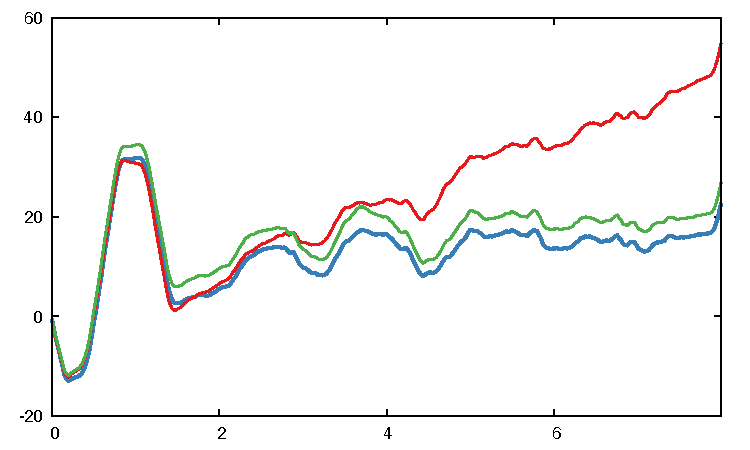
\includegraphics[width=\textwidth]{madg_data/pitch.pdf}
	    \caption{Pitch}
    \label{fig:pitch}
    \end{subfigure}
    \hfill
    \begin{subfigure}[b]{0.327\textwidth}
        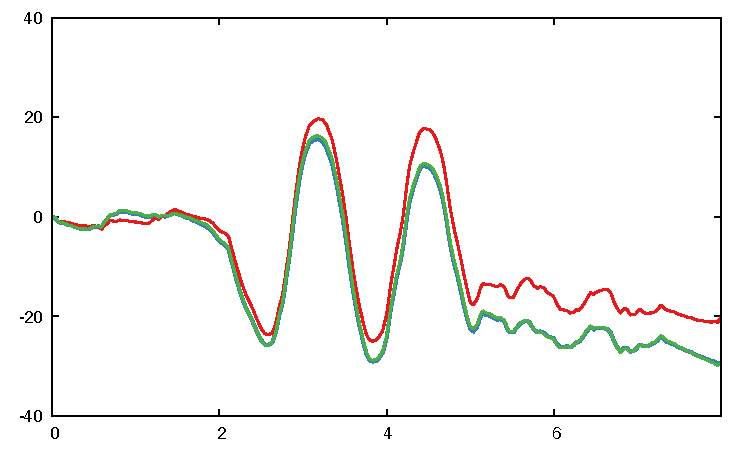
\includegraphics[width=\textwidth]{madg_data/yaw.pdf}
        \caption{Yaw}
        \label{fig:yaw}
    \end{subfigure}
    \hfill
    \begin{subfigure}[b]{0.327\textwidth}
        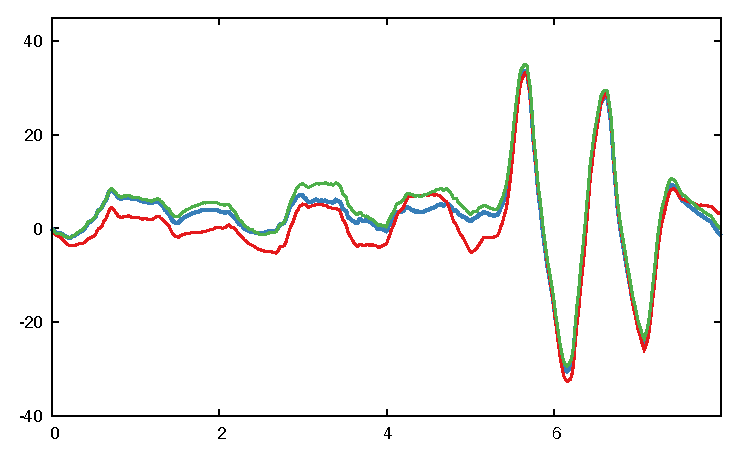
\includegraphics[width=\textwidth]{madg_data/roll.pdf}
        \caption{Roll}
        \label{fig:roll}
    \end{subfigure}
    \hfill
    \caption{Empirical results measuring the ability of InteGreat's recovered models of Orientation Estimation algorithms to identify bugs.}
    \label{fig:madg}
\end{figure*}

Note that only three lines are present in Fig.~\ref{fig:madg}.
The fourth line, the correct Matlab implementation, the blue line, is identical to lifted version of a corresponding correct C implementation.
This finding ensures InteGreat\ did not make mistakes while lifting, and was able to produce identically behaving Matlab code with respect to compiled C firmware code.
The equivalence between the two correct implementations gives us confidence in the methodology InteGreat\ introduces.

The figure depicts the same inputs to the IMU sensor of a device oscillating in pitch, yaw, then roll. \textbf{Green} is lifted by InteGreat\ from \emph{real world} firmware that contains a bug. \textbf{Blue} contains \emph{two} lines: the InteGreat\ lifted firmware recompiled to correct the gradient calculation, and \emph{a correct} Matlab implementation of Madgwick's algorithm. \textbf{Red}, however, is a compiled firmware using the \emph{faulty} C code included in Madgwick's published report. This version has accumulative error with respect to the earth's magnetic field.

Continuous equations lifted by InteGreat\ were identical to ground truth simulations in a controlled IMU sensor experiment rotating the quadcopter in 3 dimensions using 1,600 measurement points. This demonstrates our framework is able to lift correct continuous equations from discrete, machine code implementations and verify them using tools operating over the abstract domain.

\paragraph{Example of InteGreat Identifying Bugs}
\label{sec:quadcopter}

%Even the proposer of this algorithm published two variants, one C implementation in the appendix of his report and a Matlab implementation on his website after the Orientation Filter became increasingly popular for commodity drones ~\cite{}.

We next evaluate whether InteGreat\ is useful when attempting to identify bugs in firmware.
When comparing the Madgwick-provided Matlab implementation (blue) with the version recovered from the \emph{real world} firmware implementation (green), we discovered an error in the gradient of the solution surface which is calculated by multiplying the objective Function matrix and its Jacobian matrix: $\nabla F = \mathbf{J}^T(_{E}^{S}\hat{\mathbf{q}},^{E}\hat{\mathbf{b}}) \mathbf{F}(_{E}^{S}\hat{\mathbf{q}},^{E}\hat{\mathbf{b}}, ^{S}\hat{\mathbf{a}}, ^{S}\hat{\mathbf{m}})$.
Comparing the correct magnetic field components of the Objective Function with the InteGreat\ lifted version (using normalized magnetic field sensor values for simplicity):

\newcommand*{\Scale}[2][4]{\scalebox{#1}{$#2$}}%
$$
\mathbf{f}_b(_{E}^{S}\hat{\mathbf{q}},^{E}\hat{\mathbf{b}} ^{S}\hat{\mathbf{m}}) = 
\begin{bmatrix}
    2b_{x}(0.5-q_{3}^{2}-q_{4}^{2})+2b_{z}(q_{2}q_{4}-q_{1}q_{3})-m_{x}\\
    2b_{x}(q_{2}q_{3}-q_{1}q_{4})+2b_{z}(q_{1}q_{2}+q_{3}q_{4})-m_{y}\\
    2b_{x}(q_{1}q_{3}+q_{2}q_{4})+2b_{z}(0.5-q_{2}^{2}-q_{3}^{2})-m_{z}\\
\end{bmatrix}
$$

\[
\begin{aligned}
	F_4 &= ((0.5 + (- q_3 ^ 2 ) + (- q_4 ^ 2 ))  * b_x  + (q_2 * q_4  + (- q_1 * q_3 )) * b_z + (- m_x) \\
	F_5 &= (q_2 * q_3  + (- q_1 * q_4 )) * b_x + (q_3 * q_4 + q_1 * q_2) * b_z + (- m_y) \\
	F_6 &= (((0.5 + (- q_2 ^ 2)) + (- q_3 ^ 2))  * b_z  + (q_1 * q_3  + q_2 * q_4 ) * b_x + (- mz) \\
\end{aligned}
\]
\normalsize

It is clear that terms using the earth’s magnetic field ($^{E}\hat{\mathbf{b}}$) in the Objective Function have missing coefficients.\footnote{
	$b_{y}$ is not present as the earth’s magnetic field is be considered to have components in one horizontal axis and the vertical axis.}
The same errors occur in all magnetic field components of the Jacobian.
We compare only one row of the Jacobian here for simplicity:

\[
\begin{aligned}
    J_{4,1}&= (-q_3*b_z) \\
    J_{4,2}&= (q_4*b_z) \\
    J_{4,3}&= (q_3*(-2*b_x)+(-q_1*b_z)) \\
    J_{4,4}&= (q_4*(-2*b_x)+(q_2*b_z)) \\
\end{aligned}
\]
\[
\begin{aligned}
    \mathbf{J_4}(_{E}^{S}\hat{\mathbf{q}},^{E}\hat{\mathbf{b}}) &= \begin{bmatrix}
    -2b_zq_3, & 2b_zq_4, & -4b_xq_3-2b_zq_1,  & -4b_xq_4+2b_zq_2 \\
\end{bmatrix}\\
\end{aligned}
\]
\normalsize

%TODO: Is there something to be said about accumulated errors and how attacks can be made more stealthy?
After correcting all coefficients of the earth’s magnetic field ($^{E}\hat{\mathbf{b}}$) and recompiling the quad-copter firmware, the continuous equations lifted by InteGreat\ exactly matched Madgwick's Matlab implementation (blue).

We then compared the corrected equations (blue) with a \emph{third} firmware version, compiled to use Madgwick's published implementation, written in C, which is included in the original Madgwick paper (red).
We found that the published variant of the algorithm recursively feeds in previously calculated gyroscopic biases multiplied by a correction constant $\zeta$.
In contrast, existing implemented algorithms did \emph{not} perform gyroscopic bias removal and instead used dynamically calculated flux vectors of the Earth's frame in the equation's objective function.
This further confirmed InteGreat's ability to help researchers understand differences between implementations and published results.

% research question answer
By lifting compiled machine code to continuous equations using logical reasoning, it is possible to identify bugs in firmware implementations and check the validity of published results.
Validation can be performed by comparing representations which, after lifting, operate over the same domain, or by using a framework to check output equivalence, i.e. reachability, between algorithm versions.

% InteGreat's output was:
% $$
% \begin{aligned}
%     &w_{errz} = ((2 * q_1  * s_4) + (- 2 * q_2 * s_3)  + (2 * q_3 * s_2) + (- 2 * q_4 * s_1))\\
%     &w_{erry} = ((2 * q_1  * s_3)  + (2 * q_2 * s_4) + (- 2 * q_3 * s_1) + (- 2 * q_4 * s_2))\\
%     &w_{errx} = ((2 * q_1  * s_2)  + (- 2 * q_2 * s_1) + (- 2 * q_3 * s_4) + (2 * q_4 * s_3))\\
%     &w_{bz} = (w_{errz} * \zeta * \delta_t + w_{bz})\\
%     &w_{by} = (w_{erry} * \zeta * \delta_t + w_{bx})\\
%     &w_{bx} = (w_{errx} * \zeta * \delta_t + w_{by})\\
% \end{aligned}
% $$



% Taking in account the numerous different implementations of the Madgwick Orientation Filter, we consider a Madgwick Orientation Filter to be \emph{Correct} if the gradient calculation is the same as published in Madgwick's paper, and the gradient correctly updates the quaternion; \emph{Complete} if the Orientation estimation is within reasonable error range of the algorithm published by Madgwick.

% \begin{figure}
%     \centering
%     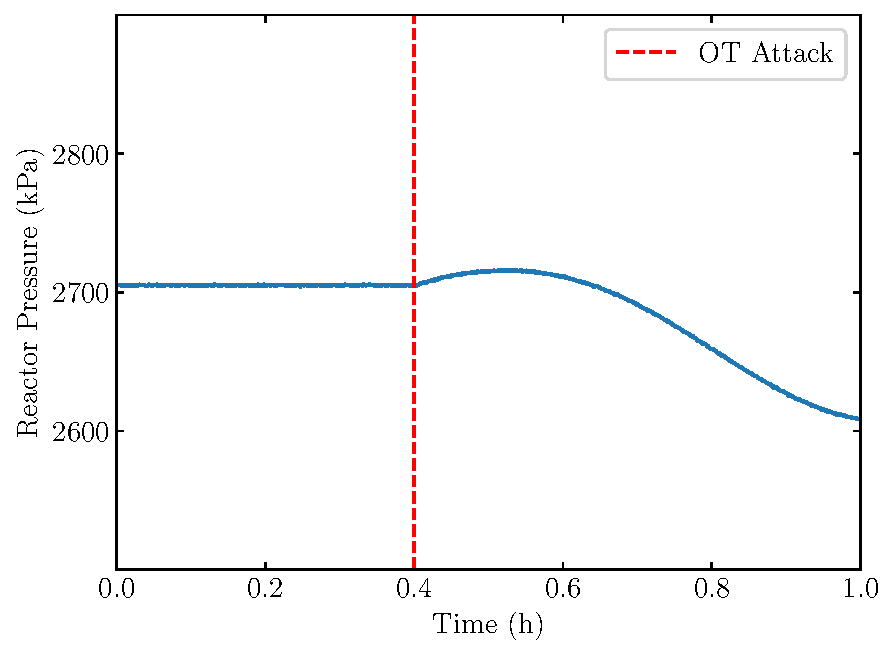
\includegraphics[width=0.4\textwidth]{plc_data/plot.pdf}
%     \caption{Simulated OT attack on the continuous equations \emph{lifted} from closed source, symbol-stripped PLC firmware.}
%     \label{fig:te_attack}
% \end{figure}





\subsection{Analyzing and Extracting Functions from PLC Firmware}
\label{sec:plc}

In this section, we demonstrate our ability to analyze continuous equation models of the firmware of a PLC (Fig.~\ref{fig:plc-stats}).
We recovered the following core model from the firmware's PID (proportional-integral-derivative) functions, where I and D are uninterpreted functions for integral and derivative, respectively:
\begin{equation}
v_{6}(
(v_{3}-v_{2})+
\frac{1}{v_{5}}
I(v_{3}-v_{2},1000t)
+
v_{1}
D(v_{3}-v_{2},1000t)
)+v_{0}+v_{7}
    \label{eqn:ideal_pid_fixcycle}
\end{equation}

For analysis in Matlab, we needed to also take into account some non-infinitesimal measure of time.
We simplified the recovered equation further via a few additional common axioms, e.g. $new\_sym = v_{3} - v_{2}$, $integ\_e\_dt = I(binds_{i0}, binds_{i1})$:
\begin{equation}
    K_{p}(
        e + 
        \frac{1}{\tau_{i}}
        \int e \mathrm{d}t
        + 
        \tau_{d}
        dv e t
    ) + b
    \label{eqn:ideal_pid_fixcycle}
\end{equation}

Eqn.~\ref{eqn:ideal_pid_fixcycle} more closely matches the traditional PID formulation, where $K_{p}$ is the proportional gain constant the ICSREF attack modified.
The other equations InteGreat\ recovered from the PLC did not require further constructed abstraction specifications.

\textbf{Discovering Additional Hardware.}
In the lifted version of the firmware, we also found an obscure scaling was applied to the sensor value for the input reactor pressure before it was supplied to Eqn.~\ref{eqn:ideal_pid_fixcycle}:

\begin{equation}
    P = 1000(((P_{digital} / 30000) - 0.0046) / 0.9876) + 2000
	\label{eqn:input-conv}
\end{equation}

\begin{figure*}
    \centering
    \begin{subfigure}[b]{0.49\textwidth}
        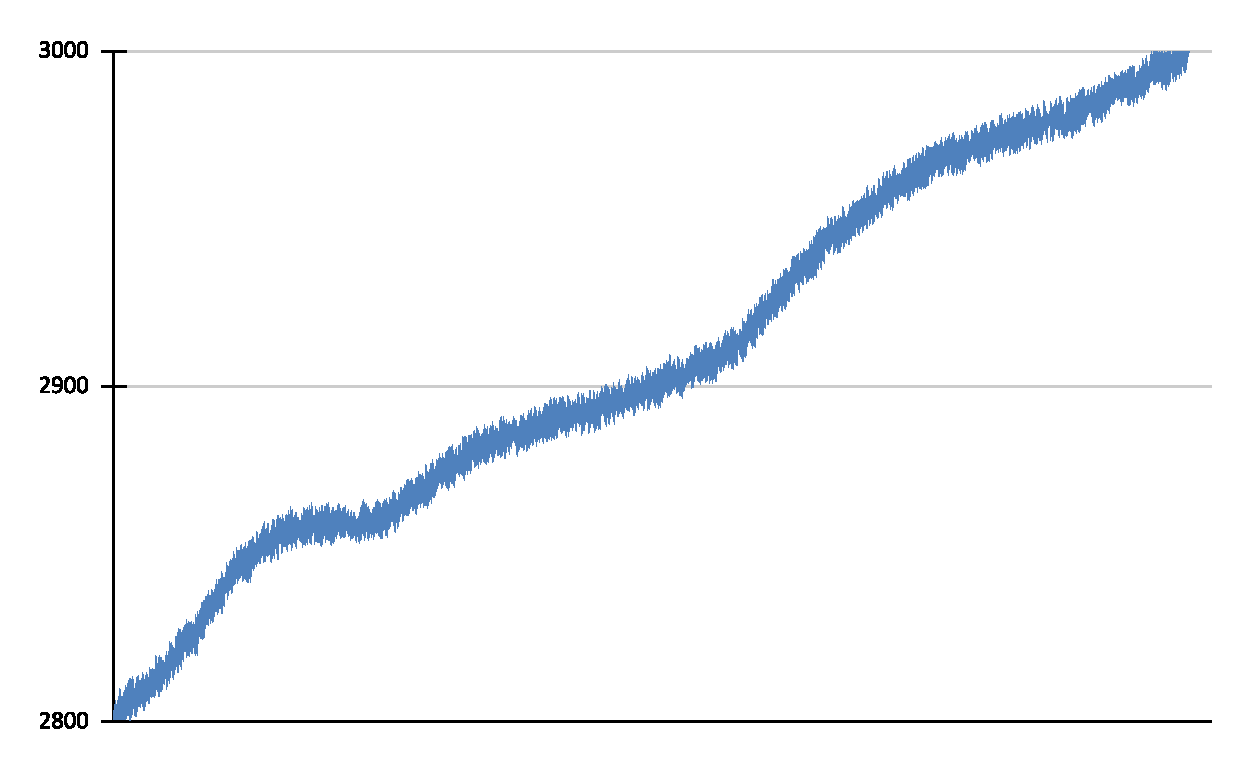
\includegraphics[width=\textwidth]{fig/plc-orig.pdf}
        \caption{Naive Attack Reproduction}
        \label{fig:orig-attack}
    \end{subfigure}
    \hfill
    \begin{subfigure}[b]{0.49\textwidth}
        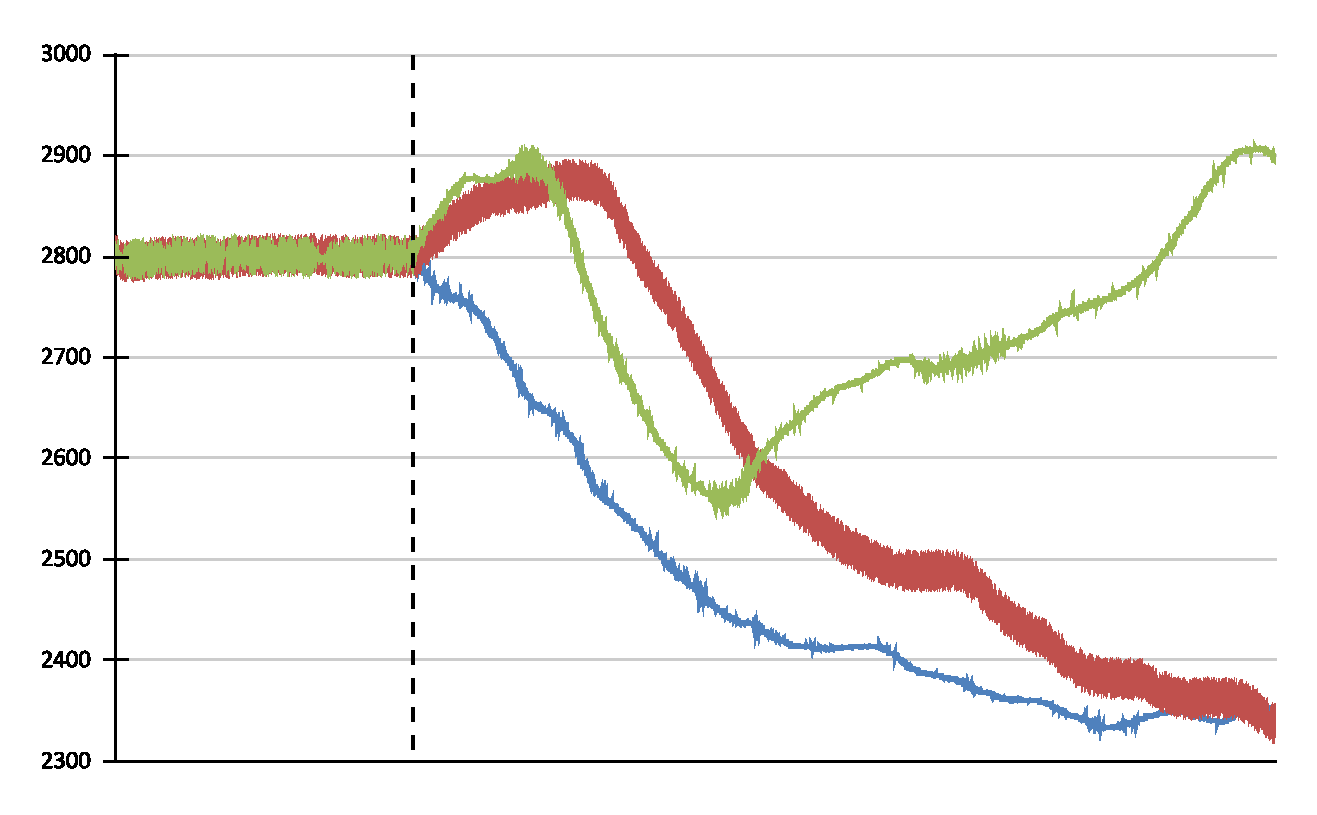
\includegraphics[width=\textwidth]{fig/dashed-plc.pdf}
	    \caption{Voltage Corrected Destabilization}
        \label{fig:noconv-attack}
    \end{subfigure}
    \hfill
	\caption{\textbf{Left}: An attempt to stage the ICSREF attack using the recovered model without taking into account the physical effects of digital-to-analog conversion. The plant shuts down upon when the reactor pressure hits 3000 kPa. \textbf{Right}: Variations of the staged attack with physical effects accounted for. The dashed line is the point at which the attack occurs (the 4 hour mark).}
    \label{fig:plc-eval}
\end{figure*}

We also were recovering the wrong value for the reactor pressure when we staged normal operation of the environmental model using our lifted equations, depicted in Fig.~\ref{fig:orig-attack}.
This led us to discover the reactor pressure (which starts at 2800 kPa in the TE simulation) was supplied to the PLC through a \emph{physical wire} connected to a separate Analog-to-Digital Converter (ADC), rather than a serial port.
The original pressure value is converted to a voltage value between 1 and 3, and then this voltage is converted back to a digital value on the physical PLC (30,000) corresponding to 3 volts.

We confirmed this was the case with the ICSREF authors.
Because of the the physical effects of the ADC being taken into account, the scaling equations applied to PLC I/O values in the Matlab environmental model used by the paper were \emph{not} the inverse of Eqn.~\ref{eqn:input-conv}.
Instead, the Matlab environmental model had no scaling to account for the ADC and the firmware \emph{implicitly} suggested the ADC was present via the scaling computation.

Even without ground truth, we were able to discover the presence of a physical ADC by analyzing a firmware's equations after lifting.
This demonstrates novel discoveries about a system's environment can be made by using InteGreat\ to analyze firmware.

\section{Precise Destabilization Attack Development}
The ICSREF attack flipped the sign on the proportional gain constant of the first of the firmware's PID calls.
By recovering the continuous equations the firmware image implemented, we were able to \emph{stage} this attack without access to the physical PLC.

A naive digital twin of the firmware's implementation, maintaining the original voltage conversions discussed above, results in Fig.~\ref{fig:orig-attack} when staging the attack.
This is because  the input and output values to the PLC's equations are affected by the scaling decided by the physical digital-to-analog and analog-to-digital converters.
This proposes the importance of a hybrid approach to modeling in the current domain of firmware rehosting~\cite{jetset,p2im,halucinator}.
While an exact emulation of the firmware's operation is desirable for dynamic analysis and testing (e.g. fuzzing), it is also necessary to verify that the I/O boundaries of the system are consistent with the physical environment or environmental model the emulation is attached to.

Moving forward with this new understanding, we were able to correctly reproduce the destabilizing effects on reactor pressure created by uploading code to the PLC (Fig.~\ref{fig:noconv-attack}).
\textbf{Red} represents the original PLC firmware behavior from the ICSREF paper.
However, notice that the paper included an unexplained positive bump at the point of attack.
Lifted equations allow us to explore an idealized model of the firmware's implementation: by removing all scaling operations from Matlab and the recovered model, we attained the line in \textbf{Blue}.
In doing so, we discovered exactly how much the ADC voltage conversion affects the cyberphysical system's dynamics.
The \textbf{Green} line represents a case where the attack \emph{did not} occur but control over the reactor pressure is given to the PLC (with ADC scaling).
This scaling makes the pressure of the plant far less stable, a feature of the system not addressed in the original ICSREF paper.

Using InteGreat\ we were able to both reproduce and verify an existing attack on a PLC, develop an idealized model of the PID controller's operation, and isolate the effects of the physical environment on the system's dynamics.
This demonstrates our approach is useful for the reproduction and analysis of attacks and models for cyberphysical systems.

Because the recovered models of the PLC's control equations are general, it is possible to compute reachable values for any variety of system states and environmental models.
Therefore, the recovered equations are of value in \emph{precisely} destabilizing the plant's reactor pressure while maintaining the appearance of correct behavior, similar to stuxnet~\cite{baezner2017stuxnet}.

\section{Discussion}

Informed by both the Jetset and Edact-Ray works, InteGreat adopts an opinionated perspective on the challenges facing binary program analysis.
It attempts to address universal and necessary limitations to abstract interpretation, such as the modeling of microarchitectural semantics and state explosion, by applying the well-worn technique of wrapping these complexities in a layer of indirection, and then automates the construction of this indirection.
While this alleviates the \emph{immediate} difficulties involved in inferring loop invariants and pointer analysis, InteGreat also has the explicit limitation of requiring users to leave these semantics undefined or provide their own formulae for resolution.
We therefore see two potential future applications of InteGreat:

\paragraph{Sub-System High Level Emulator Extraction}
InteGreat's recovered models can also be used as a rudimentary form of firmware rehosting where only algorithms are needed.
As demonstrated in our PLC and Quadcopter experiments, InteGreat can provide control system verifiers with additional, real-world evaluation targets.
Lifting rules can also be specified independently of the software itself, and extracted functions could serve as a contract that the concrete system is implemented according to some model.

\paragraph{Lifting Libraries}
By incorporating an object-oriented approach for abstraction specifications, the InteGreat framework is also able to continually expand its base of knowledge.
A given set of lifting rules can be written and then shared, similar to a library, for the analysis of wide ranges of firmware binaries.
These libraries may also be generated via automated methods, and serve as a compressed encoding of more complex inference procedures.

\paragraph{Bottom-up Verification}
InteGreat does not solve the \emph{internal} or \emph{external} semantic problems posed in Section~\ref{sec:jetset-limitations} or the more general problem of missing information in a system's specification.
Instead, the system attempts to provide a better interface for management of this problems.
It does so by making no assumptions about the underlying semantics of the system, building a model of the system from the ground up by starting with the implementation, rather than a mathematical model.

In providing an interface for a more abstract representation the system during symbolic execution, InteGreat is able to rely on additional input for undefined or undecidable cases and extract useful models in cases where no such additional information is required or feasible to provide.
InteGreat thereby alleviates the need to treat complex systems as complete black-boxes,\footnote{The dangers of making representational assumptions were demonstrated in Chapter~\ref{chap:info}.} and instead attempts to restrict the use of black-boxes to cases where information on the system is legitimately missing.


\section{Summary}

The work presented in this chapter empirically demonstrates that traditional top-down approaches to verification can underestimate the complexity of firmware implementations.
Instead of \emph{only} working from mathematical models of a specific implemented system, we propose the additional application of careful, logic-based function extraction.
From this point of view, it is possible to define the system at arbitrary levels of granularity while ensuring that the provided representation for verification is accurate to the system under study.
For this purpose, we developed a system that applies logic-based function extraction to recover continuous equations from symbol-stripped binary firmware.
Through the analysis of two real world systems, a quad-copter and PLC, we were able to demonstrate such an approach's ability to find differences between published, high-level representations and low-level system representations.
We were also able to elucidate otherwise unknowable features of a system under study, such as physical ADCs and the effects of their value representation on the system's dynamics.

\chapter{Conclusions}
\label{chap:conclusion}


% }}}

% {{{ back matter
\bibliographystyle{IEEE_ECE}
\bibliography{references}  % Put references in BibTeX format in thesisrefs.bib.

\appendix

\backmatter

% }}}

\end{document}
